\NewExpandableDocumentCommand{\TeXturedVERSION}{}{1.2.0} 


%% Enable built-in LaTeX support for PDF/A compliance (must be before `\documentclass`)
\DocumentMetadata{lang=en, pdfversion=1.7, pdfstandard=A-2u}
%%% PDF/A compliance - glyph to Unicode mappings

%% NOTE: metadata are set up using the `hyperref` package in `preamble/general/hyperref.tex`

%% WARN: `pdfx` package is SUPERSEDED by built-in LaTeX support for PDF/A
%%       However, in case additional fonts are used, some glyphs may not be covered
%%       by default Unicode mappings, in which case they need to be mapped to Unicode
%%       code points manually (see below for GUIDE and examples).

%%% GUIDE: How to add missing unicode mappings for glyphs
%%
%% Consider following part of VeraPDF output for a non-compliant PDF:
%%   <rule specification="ISO 19005-2:2011" clause="6.2.11.7.2" testNumber="1" status="failed" passedChecks="0" failedChecks="1">
%%     <description>The Font dictionary of all fonts shall define the map of all used character codes to Unicode values,
%%                  either via a ToUnicode entry, or other mechanisms as defined in ISO 19005-2, 6.2.11.7.2.</description>
%%     <object>Glyph</object>
%%     <test>toUnicode != null</test>
%%     <check status="failed">
%%       <context>root/document[0]/pages[58](1323 0 obj PDPage)/contentStream[0](1324 0 obj PDContentStream)
%%                                          /operators[654]/usedGlyphs[0](RMTQUN+MSAM10 RMTQUN+MSAM10 57 0  0)</context>
%%       <errorMessage>The glyph can not be mapped to Unicode</errorMessage>
%%     </check>
%%   </rule>
%%
%% This means that some glyph on page 59 (indicated by a 0-based index `pages[58]`)
%% is missing a Unicode mapping. To fix this, we need to find the name of the glyph,
%% and provide a Unicode mapping for it. For further instructions how to proceed see
%% `preamble/pdfA-compliance/LaTeX-find-glyph-name/LaTeX-find-glyph-name.tex`.

\RequirePackage{iftex}
\ifluatex % only for luaLaTeX (sourced by default for pdfLaTeX)
    \RequirePackage{luatex85}
    %%% PDF/A compliance - glyph to Unicode mappings

%% NOTE: metadata are set up using the `hyperref` package in `preamble/general/hyperref.tex`

%% WARN: `pdfx` package is SUPERSEDED by built-in LaTeX support for PDF/A
%%       However, in case additional fonts are used, some glyphs may not be covered
%%       by default Unicode mappings, in which case they need to be mapped to Unicode
%%       code points manually (see below for GUIDE and examples).

%%% GUIDE: How to add missing unicode mappings for glyphs
%%
%% Consider following part of VeraPDF output for a non-compliant PDF:
%%   <rule specification="ISO 19005-2:2011" clause="6.2.11.7.2" testNumber="1" status="failed" passedChecks="0" failedChecks="1">
%%     <description>The Font dictionary of all fonts shall define the map of all used character codes to Unicode values,
%%                  either via a ToUnicode entry, or other mechanisms as defined in ISO 19005-2, 6.2.11.7.2.</description>
%%     <object>Glyph</object>
%%     <test>toUnicode != null</test>
%%     <check status="failed">
%%       <context>root/document[0]/pages[58](1323 0 obj PDPage)/contentStream[0](1324 0 obj PDContentStream)
%%                                          /operators[654]/usedGlyphs[0](RMTQUN+MSAM10 RMTQUN+MSAM10 57 0  0)</context>
%%       <errorMessage>The glyph can not be mapped to Unicode</errorMessage>
%%     </check>
%%   </rule>
%%
%% This means that some glyph on page 59 (indicated by a 0-based index `pages[58]`)
%% is missing a Unicode mapping. To fix this, we need to find the name of the glyph,
%% and provide a Unicode mapping for it. For further instructions how to proceed see
%% `preamble/pdfA-compliance/LaTeX-find-glyph-name/LaTeX-find-glyph-name.tex`.

\RequirePackage{iftex}
\ifluatex % only for luaLaTeX (sourced by default for pdfLaTeX)
    \RequirePackage{luatex85}
    %%% PDF/A compliance - glyph to Unicode mappings

%% NOTE: metadata are set up using the `hyperref` package in `preamble/general/hyperref.tex`

%% WARN: `pdfx` package is SUPERSEDED by built-in LaTeX support for PDF/A
%%       However, in case additional fonts are used, some glyphs may not be covered
%%       by default Unicode mappings, in which case they need to be mapped to Unicode
%%       code points manually (see below for GUIDE and examples).

%%% GUIDE: How to add missing unicode mappings for glyphs
%%
%% Consider following part of VeraPDF output for a non-compliant PDF:
%%   <rule specification="ISO 19005-2:2011" clause="6.2.11.7.2" testNumber="1" status="failed" passedChecks="0" failedChecks="1">
%%     <description>The Font dictionary of all fonts shall define the map of all used character codes to Unicode values,
%%                  either via a ToUnicode entry, or other mechanisms as defined in ISO 19005-2, 6.2.11.7.2.</description>
%%     <object>Glyph</object>
%%     <test>toUnicode != null</test>
%%     <check status="failed">
%%       <context>root/document[0]/pages[58](1323 0 obj PDPage)/contentStream[0](1324 0 obj PDContentStream)
%%                                          /operators[654]/usedGlyphs[0](RMTQUN+MSAM10 RMTQUN+MSAM10 57 0  0)</context>
%%       <errorMessage>The glyph can not be mapped to Unicode</errorMessage>
%%     </check>
%%   </rule>
%%
%% This means that some glyph on page 59 (indicated by a 0-based index `pages[58]`)
%% is missing a Unicode mapping. To fix this, we need to find the name of the glyph,
%% and provide a Unicode mapping for it. For further instructions how to proceed see
%% `preamble/pdfA-compliance/LaTeX-find-glyph-name/LaTeX-find-glyph-name.tex`.

\RequirePackage{iftex}
\ifluatex % only for luaLaTeX (sourced by default for pdfLaTeX)
    \RequirePackage{luatex85}
    \input{glyphtounicode.tex} % probably not loaded automatically for luatex
    \pdfgentounicode=1         % probably disabled by default for luatex
\fi

%% Enable in case some glyphs are missing from imported PDF figures
\pdfinclusioncopyfonts=1

%% Additional Unicode mappings for mathematical symbols (provided by `pdfx`)
%% https://gist.github.com/literalplus/045c4d090e2fe742157b4c903a984d24
\input{glyphtounicode-cmr.tex} % <- /usr/share/texmf-dist/tex/latex/pdfx/glyphtounicode-cmr.tex
% \input{glyphtounicode-ntx.tex} % <- /usr/share/texmf-dist/tex/latex/pdfx/glyphtounicode-ntx.tex


%%% Additional Unicode mappings for various extra glyphs

%% Glyphs: double brackets (of various sizes)
%% name of glyph found in /usr/share/texmf-dist/fonts/afm/public/stmaryrd/stmary5.afm
\pdfglyphtounicode{llbracket}{27E6} % https://codepoints.net/U+27E6
\pdfglyphtounicode{rrbracket}{27E7} % https://codepoints.net/U+27E7
\pdfglyphtounicode{largellbracket}{27E6 FE01} % variants according to size
\pdfglyphtounicode{largerrbracket}{27E7 FE01} % ... ... .. ....
\pdfglyphtounicode{Largellbracket}{27E6 FE02} % ... ... .. ....
\pdfglyphtounicode{Largerrbracket}{27E7 FE02} % ... ... .. ....
\pdfglyphtounicode{LARGEllbracket}{27E6 FE03} % ... ... .. ....
\pdfglyphtounicode{LARGErrbracket}{27E7 FE03} % ... ... .. ....
\pdfglyphtounicode{hugellbracket} {27E6 FE04} % ... ... .. ....
\pdfglyphtounicode{hugerrbracket} {27E7 FE04} % ... ... .. ....
\pdfglyphtounicode{Hugellbracket} {27E6 FE05} % ... ... .. ....
\pdfglyphtounicode{Hugerrbracket} {27E7 FE05} % ... ... .. ....
\pdfglyphtounicode{Hugellbrackettop}{23A5 23A1} % separate top, middle, bottom
\pdfglyphtounicode{Hugellbracketex} {23A5 23A2} % ... ... .. ....
\pdfglyphtounicode{Hugellbracketbot}{23A6 23A3} % ... ... .. ....
\pdfglyphtounicode{Hugerrbrackettop}{23A4 23A2} % ... ... .. ....
\pdfglyphtounicode{Hugerrbracketex} {23A5 23A2} % ... ... .. ....
\pdfglyphtounicode{Hugerrbracketbot}{23A6 23A2} % ... ... .. ....

%% Glyph: short minus
\pdfglyphtounicode{axisshort}{2212} % short minus -> minus https://codepoints.net/U+2212

%%% TODO: maybe use `\pdfstringdefDisableCommands` for something (in PDF metadata?)
 % probably not loaded automatically for luatex
    \pdfgentounicode=1         % probably disabled by default for luatex
\fi

%% Enable in case some glyphs are missing from imported PDF figures
\pdfinclusioncopyfonts=1

%% Additional Unicode mappings for mathematical symbols (provided by `pdfx`)
%% https://gist.github.com/literalplus/045c4d090e2fe742157b4c903a984d24
\input{glyphtounicode-cmr.tex} % <- /usr/share/texmf-dist/tex/latex/pdfx/glyphtounicode-cmr.tex
% \input{glyphtounicode-ntx.tex} % <- /usr/share/texmf-dist/tex/latex/pdfx/glyphtounicode-ntx.tex


%%% Additional Unicode mappings for various extra glyphs

%% Glyphs: double brackets (of various sizes)
%% name of glyph found in /usr/share/texmf-dist/fonts/afm/public/stmaryrd/stmary5.afm
\pdfglyphtounicode{llbracket}{27E6} % https://codepoints.net/U+27E6
\pdfglyphtounicode{rrbracket}{27E7} % https://codepoints.net/U+27E7
\pdfglyphtounicode{largellbracket}{27E6 FE01} % variants according to size
\pdfglyphtounicode{largerrbracket}{27E7 FE01} % ... ... .. ....
\pdfglyphtounicode{Largellbracket}{27E6 FE02} % ... ... .. ....
\pdfglyphtounicode{Largerrbracket}{27E7 FE02} % ... ... .. ....
\pdfglyphtounicode{LARGEllbracket}{27E6 FE03} % ... ... .. ....
\pdfglyphtounicode{LARGErrbracket}{27E7 FE03} % ... ... .. ....
\pdfglyphtounicode{hugellbracket} {27E6 FE04} % ... ... .. ....
\pdfglyphtounicode{hugerrbracket} {27E7 FE04} % ... ... .. ....
\pdfglyphtounicode{Hugellbracket} {27E6 FE05} % ... ... .. ....
\pdfglyphtounicode{Hugerrbracket} {27E7 FE05} % ... ... .. ....
\pdfglyphtounicode{Hugellbrackettop}{23A5 23A1} % separate top, middle, bottom
\pdfglyphtounicode{Hugellbracketex} {23A5 23A2} % ... ... .. ....
\pdfglyphtounicode{Hugellbracketbot}{23A6 23A3} % ... ... .. ....
\pdfglyphtounicode{Hugerrbrackettop}{23A4 23A2} % ... ... .. ....
\pdfglyphtounicode{Hugerrbracketex} {23A5 23A2} % ... ... .. ....
\pdfglyphtounicode{Hugerrbracketbot}{23A6 23A2} % ... ... .. ....

%% Glyph: short minus
\pdfglyphtounicode{axisshort}{2212} % short minus -> minus https://codepoints.net/U+2212

%%% TODO: maybe use `\pdfstringdefDisableCommands` for something (in PDF metadata?)
 % probably not loaded automatically for luatex
    \pdfgentounicode=1         % probably disabled by default for luatex
\fi

%% Enable in case some glyphs are missing from imported PDF figures
\pdfinclusioncopyfonts=1

%% Additional Unicode mappings for mathematical symbols (provided by `pdfx`)
%% https://gist.github.com/literalplus/045c4d090e2fe742157b4c903a984d24
\input{glyphtounicode-cmr.tex} % <- /usr/share/texmf-dist/tex/latex/pdfx/glyphtounicode-cmr.tex
% \input{glyphtounicode-ntx.tex} % <- /usr/share/texmf-dist/tex/latex/pdfx/glyphtounicode-ntx.tex


%%% Additional Unicode mappings for various extra glyphs

%% Glyphs: double brackets (of various sizes)
%% name of glyph found in /usr/share/texmf-dist/fonts/afm/public/stmaryrd/stmary5.afm
\pdfglyphtounicode{llbracket}{27E6} % https://codepoints.net/U+27E6
\pdfglyphtounicode{rrbracket}{27E7} % https://codepoints.net/U+27E7
\pdfglyphtounicode{largellbracket}{27E6 FE01} % variants according to size
\pdfglyphtounicode{largerrbracket}{27E7 FE01} % ... ... .. ....
\pdfglyphtounicode{Largellbracket}{27E6 FE02} % ... ... .. ....
\pdfglyphtounicode{Largerrbracket}{27E7 FE02} % ... ... .. ....
\pdfglyphtounicode{LARGEllbracket}{27E6 FE03} % ... ... .. ....
\pdfglyphtounicode{LARGErrbracket}{27E7 FE03} % ... ... .. ....
\pdfglyphtounicode{hugellbracket} {27E6 FE04} % ... ... .. ....
\pdfglyphtounicode{hugerrbracket} {27E7 FE04} % ... ... .. ....
\pdfglyphtounicode{Hugellbracket} {27E6 FE05} % ... ... .. ....
\pdfglyphtounicode{Hugerrbracket} {27E7 FE05} % ... ... .. ....
\pdfglyphtounicode{Hugellbrackettop}{23A5 23A1} % separate top, middle, bottom
\pdfglyphtounicode{Hugellbracketex} {23A5 23A2} % ... ... .. ....
\pdfglyphtounicode{Hugellbracketbot}{23A6 23A3} % ... ... .. ....
\pdfglyphtounicode{Hugerrbrackettop}{23A4 23A2} % ... ... .. ....
\pdfglyphtounicode{Hugerrbracketex} {23A5 23A2} % ... ... .. ....
\pdfglyphtounicode{Hugerrbracketbot}{23A6 23A2} % ... ... .. ....

%% Glyph: short minus
\pdfglyphtounicode{axisshort}{2212} % short minus -> minus https://codepoints.net/U+2212

%%% TODO: maybe use `\pdfstringdefDisableCommands` for something (in PDF metadata?)


%% NOTE: Choose the desirable page layout version (electronic vs print)
\documentclass[12pt,a4paper]{report}                      % single-side (electronic)
% \documentclass[12pt,a4paper,openright,twoside]{report}  % two-sided (for printing)

%% Set some toggle flags to control some of the document properties
%% Define some toggle flags

\newif\ifFANCY       %% whether to enable some more fancy stylistic choices
\newif\ifWIP         %% whether to enable debug commands, todos, etc.
\newif\ifEXTRAMARGIN %% whether WIP mode has extra right margin
\newif\ifCENSOR      %% whether to censor denoted passages

\FANCYtrue        %% by default, enable fancy features

% \FANCYfalse % disable some of the more fancy stylistic choices
%% NOTE: Comment out the following lines for the final version
%\WIPtrue            % THIS IS A WORK-IN-PROGRESS VERSION
% \EXTRAMARGINtrue  % add extra right margin in WIP version (for notes/corrections)
%\CENSORtrue         % THIS IS A CENSORED VERSION

%% Preamble - data, packages, macros, and more
%%% Preamble

%% Data about the document, like title, author, etc.
%% Thesis type: bachelor, master, doctoral
\NewExpandableDocumentCommand{\ThesisType}{}{master}

%% Thesis title (exactly as in the formal assignment)
\NewExpandableDocumentCommand{\ThesisTitle}{}{Testing and Validation of coupled atmospheric solver PALM and FAST for a Enercon Turbine}
%% Plaintext version for PDF metadata, uncomment if needed (defauls to \ThesisTitle)
\NewExpandableDocumentCommand{\ThesisTitlePlaintext}{}{TeXtured Manual \TeXturedVERSION}
%% Thesis title (if custom formatting is needed for the title page, defauls to \ThesisTitle)
\NewExpandableDocumentCommand{\ThesisTitleFront}{}{
    \ThesisTitle
}

%% Author of the thesis
\NewExpandableDocumentCommand{\ThesisAuthor}{}{Aravind Venkatachalapathy}
%% Plaintext version for PDF metadata, uncomment if needed (defauls to \ThesisAuthor)
\NewExpandableDocumentCommand{\ThesisAuthorPlaintext}{}{Aravind Venkatachalapathy}

%% Year when the thesis is submitted
\NewDocumentCommand{\YearSubmitted}{}{2025}
%% Year of the last revision, uncomment if it is different from \YearSubmitted
% \NewDocumentCommand{\YearRevision}{}{2025}

%% University
\NewDocumentCommand{\University}{}{Hochschule Flensburg}

%% Name of the department or institute, where the work was officially assigned
%% (according to the Organizational Structure of MFF UK in English,
%% or a full name of a department outside MFF)
\NewDocumentCommand{\Department}{}{Wind Energy Technology Institute}

%% Is it a Department (katedra), or an Institute (ústav)?
\NewDocumentCommand{\DeptType}{}{Institute}

%% Thesis supervisor: name, surname and titles
\NewDocumentCommand{\Supervisor}{}{\textcolor{red}{David, Schlipf, and Dr. Ing.}}
%% Thesis co-supervisor: name, surname and titles (uncomment if applicable)
% \NewDocumentCommand{\CoSupervisor}{}{Name, Surname, and Titles}

%% Supervisor's department/institute (again according to Organizational structure of MFF)
\NewDocumentCommand{\SupervisorsDepartment}{}{\textcolor{red}{Supervisor's Department/Institute}}

%% Study programme and specialization
\NewDocumentCommand{\StudyProgramme}{}{\textcolor{red}{Study Programme}}

%% Abstract (recommended length around 80-200 words; this is not a copy of your thesis assignment!)
\NewDocumentCommand{\Abstract}{}{%
    \textcolor{red}{Write abstract here.}
}

%% Subject (short description for PDF metadata)
\NewExpandableDocumentCommand{\Subject}{}{%
    Write subject here.
}

%% Keywords (about 3-7)
%\NewExpandableDocumentCommand{\Keywords}{}{%
    %\textcolor{red}{Manual, Demo, Draft, WIP}
%}
%% Plaintext version for PDF metadata, uncomment if needed (defauls to \Keywords)
%\NewExpandableDocumentCommand{\KeywordsPlaintext}{}{%
    %Manual, Demo, Draft, WIP
%}


%% DEBUG: various helper debug goodies
%% Include only listed files
%% NOTE: ignored if the document is not in WIP mode, or if the argument is empty
\NewDocumentCommand{\includeonlysmart}{m}{
    \ifWIP                              % ignore if not WIP
        \IfBlankF{#1}{\includeonly{#1}} % ignore if empty argument
    \fi
}

%% Draw black "slugs" whenever a line overflows, so that we can spot it easily
\ifWIP
    \overfullrule=1mm
    \ifluatex % only for luaLaTeX
        % \usepackage{lua-visual-debug} % helper for space tweaking
    \fi
\fi

%% Censoring
\usepackage{censor}
\ifCENSOR % censor package censors by default
    % do nothing if censoring requested
\else
    \StopCensoring % disable censoring
\fi

\usepackage[pagewise]{lineno} % line numbers for drafts

\newif\ifDebugLineNumbers
%% NOTE: Uncomment out the following line to show line numbers
% \DebugLineNumberstrue % show line numbers (by default disabled)

\ifDebugLineNumbers
    \ifWIP
        \linenumbers
        \renewcommand{\linenumberfont}{\normalfont\footnotesize\ttfamily\color{black!15}}
        \setlength\linenumbersep{1em}
    \fi
\fi

\usepackage{silence} % filter out unwanted warnings

\WarningFilter{latex}{Marginpar on page} % ignore "Marginpar on page ___ moved"


%% Colors
%% Colors
\usepackage[rgb,table]{xcolor} % color facilities

%% TODO: slightly darker gray color for "optional" words
\definecolor{ChapterNumberColor}{gray}{0.88}
\definecolor{HeaderColor}{gray}{0.35}
\definecolor{HeaderRuleColor}{gray}{0.75}
\definecolor{CiteColor}{RGB}{127,230,252}
\definecolor{LinkColor}{RGB}{255,127,100}
\definecolor{UrlColor}{RGB}{100,127,255}

\definecolor{Gray10}{gray}{0.1}
\definecolor{Gray20}{gray}{0.2}
\definecolor{Gray30}{gray}{0.3}
\definecolor{Gray40}{gray}{0.4}
\definecolor{Gray50}{gray}{0.5}
\definecolor{Gray60}{gray}{0.6}
\definecolor{Gray70}{gray}{0.7}
\definecolor{Gray80}{gray}{0.8}
\definecolor{Gray90}{gray}{0.9}

\definecolor{LightGrayFill}{gray}{0.97}


%% Typesetting, figures, tables, etc.
%%% Typesetting, figures, tables, etc.

\ifpdftex % only for pdfLaTeX
    \usepackage[T1]{fontenc} % better support for accented characters
\fi
\usepackage{lmodern}  % Latin Modern fonts
\usepackage{romanbar} % Roman numerals with bars, provides `\Romanbar{...}`

%% slightly more breathing space between lines
\linespread{1.05}\selectfont

%% Commands for accessing extra Latin Modern fonts
%%     - `sbc` - sans bold condensed
%%     - `sfe` - sans serif extended (font family `lmssq` for "Latin Modern Sans Serif Quotation")
%% https://www.tug.org/pracjourn/2006-1/robertson/robertson.pdf
\NewDocumentCommand{\sbcseries}{}{\sffamily\fontseries{sbc}\selectfont}
\NewDocumentCommand{\sfefamily}{}{\fontfamily{lmssq}\selectfont}
\DeclareTextFontCommand{\textsbc}{\sbcseries}
\DeclareTextFontCommand{\textsfe}{\sfefamily}

%% use slanted shape for emphasis `\emph{...}`, and for nested emphasis use italics
\DeclareEmphSequence{\slshape,\itshape}

\usepackage{microtype}           % improve typography
\DisableLigatures[-]{family=tt*} % disable ligatures in typewriter font
\usepackage{parskip}             % no paragraph indentation
\usepackage{csquotes}            % context-sensitive quotation facilities

%% Enumerate/itemize environments
\usepackage[alwaysadjust,neverdecrease]{paralist}   % improved enumerate and itemize
\setdefaultleftmargin{1.87em}{1.7em}{1.5em}{1em}{1em}{1em}
\setdefaultitem{$\bullet$}{\textbullet}{\textasteriskcentered}{\textperiodcentered}
\setdefaultenum{\bfseries (1)}{\bfseries (a)}{\bfseries (i)}{A.}

%% Configuration of figures, tables, captions, ...

%% Use same numbering for figures, tables, and equations
\makeatletter
\let\c@figure\c@table
\let\c@equation\c@table
\makeatother

%%% Graphics
\usepackage{graphicx}   % embedding of pictures
\graphicspath{          % default paths to figures
    {./figures/}
    {./figures/Inkscape/}
    {./frontmatter/img/}
}
%% Macro for appending to the graphics path
\ExplSyntaxOn
\NewDocumentCommand{\appendtographicspath}{m}{
    \tl_if_exist:cF { Ginput@path } { \tl_new:c { Ginput@path } }
    \tl_gput_right:cn {Ginput@path} { #1 }
}
\ExplSyntaxOff

%%% Tables
\usepackage{adjustbox}      % center big tables
\usepackage{array}          % custom column types in tables
\usepackage{booktabs}       % improved horizontal lines in tables

%% Increase default vertical space between rows in tables (default is 1.0)
\renewcommand*{\arraystretch}{1.1}

% HACK: `ninecolors` is needed for `tabularray`, but fails to load with
%       rgb color model -> see https://tex.stackexchange.com/a/614702
\selectcolormodel{natural}  % temporarily switch to natural color model
\usepackage{ninecolors}     % now we can load `ninecolors` package
\selectcolormodel{rgb}      % switch back to RGB color model

\usepackage{tabularray}     % advanced LaTeX tables
\usepackage{codehigh}       % verbatim in tables (with `\fakeverb` macro)
\UseTblrLibrary{amsmath, booktabs, siunitx} % load libraries for `tabularray`


%% Does \centering automatically, provides side captions (`\fcapside`) and much more
%% Inspired by https://collaborating.tuhh.de/m21/public/theses/itt-latex-template
\usepackage{floatrow}
\floatsetup{ % for all floats
    footnoterule = none,
    footposition = bottom,
}
\floatsetup[figure]{
    capbesideposition = right,
    capbesidesep = quad,
}

%% If you want to position the caption above the figure, use the following
% \floatsetup[table]{
%     style = plaintop, % caption always above, no matter where \caption is called
% }

%% Set caption width to be the same as the table width
% \floatsetup[longtable]{LTcapwidth=table} % https://tex.stackexchange.com/a/345772/120853

\usepackage{caption}    % customizing captions in floating environments
\usepackage{subcaption}

% \DeclareCaptionLabelSeparator{slash}{~/~} % `␣/␣` between label and caption
\DeclareCaptionLabelSeparator{slash}{\hspace{0.25em}/\hspace{0.25em}} % `␣/␣` between label and caption
\captionsetup{
    format        = plain,  % no hanging indent
    indention     = 0.6em,  % but still slightly indent the caption
    % format        = hang,   % alternative: hanging indent
    font          = small,
    labelfont     = {sf,bf},
    labelsep      = slash,
    labelformat   = simple,
    tableposition = bottom,
    parskip       = .3\baselineskip plus 1pt,
}

\makeatletter
% Make this new length and indent, same length as regular caption indent:
\newlength{\floatfootruleindent}
\setlength{\floatfootruleindent}{\caption@indent}% Set the new length
% A bit hacky; introduce a rule underneath caption if \floatfoot is called:
\renewcommand*{\floatfootskip}{2pt\color{Gray50}\hspace{\floatfootruleindent}\hrulefill}%
\makeatother

\DeclareCaptionFont{ftfont}{%
    \scriptsize%
    \color{Gray60}%
    \sffamily\raggedleft%
}
\captionsetup[floatfoot]{
    footfont=ftfont, % https://tex.stackexchange.com/q/9547/120853
}

%%% You can change the justification of all side-captions here
% \captionsetup[capbesidefigure]{
%     % When using sidecaptions, the linewidth can be rather small and awkward breaks and
%     % many underfull hboxes occur. Therefore, raggedright.
%     justification=raggedright,
% }
%
% \captionsetup[subfigure]{%
%     labelformat=simple,% 'parens' uses parantheses, 'brace' just the right one
%     labelsep=slash,%
%     labelfont={sf,bf},%
%     list=off,% list=off removes subfigures from LoF
% }%
%
% \captionsetup[subtable]{%
%     labelformat=simple,% 'parens' uses parantheses, 'brace' just the right one
%     labelsep=slash,%
%     labelfont={sf,bf},%
%     list=off,% list=off removes subfigures from LoF
% }%

%% Change counter from Arabic number to letter:
\renewcommand*{\theContinuedFloat}{\alph{ContinuedFloat}}


%% Hyperlinks, PDF metadata
%% Hyperlinks, PDF metadata
%\usepackage[allowmove]{url}
\usepackage[hyphens]{url}  % allows line breaks at hyphens in URLs
\usepackage{hyperref}   % clickable links and metadata
\usepackage{nameref}    % cross-referencing by name
\usepackage{bookmark}   % more control over PDF bookmarks

%% Fallbacks for PDF metadata commands
\ProvideExpandableDocumentCommand{\ThesisAuthorPlaintext}{}{\ThesisAuthor}
\ProvideExpandableDocumentCommand{\ThesisTitlePlaintext}{}{\ThesisTitle}
\ProvideExpandableDocumentCommand{\KeywordsPlaintext}{}{\Keywords}

\hypersetup{
    linktoc=all,         % whole entry in TOC is clickable link
    pdfborder={0 0 0},   % to disable borders/frames around links
    pdflinkmargin=1.0pt, % extra link area around the text box (default 1pt)
    citebordercolor=CiteColor,
    linkbordercolor=LinkColor,
    urlbordercolor=UrlColor,
    % PDF metadata
    pdfauthor=\ThesisAuthorPlaintext,
    pdftitle=\ThesisTitlePlaintext,
    pdfsubject=\Subject,
    pdfkeywords=\KeywordsPlaintext,
    pdfcreator={LaTeX with hyperref, and biblatex/biber},
    pdfdisplaydoctitle, % https://tex.stackexchange.com/a/435434/120853
}
\bookmarksetup{
    numbered, % include chapter/section numbers in PDF outline
    open, openlevel=1, % expand bookmarks to level 1 (chapters)
}



\urlstyle{same}        % keep font same as surrounding text

% Allow breaks at more characters
\makeatletter
\g@addto@macro{\UrlBreaks}{\do\/\do-}
\makeatother


%% NOTE: look of references, hyperlinks, and citations is customized
%%       mainly in `preamble/hacks/custom-reference-boxes.tex`


%% Miscellaneous commands/macros
%% User macros

%% TeXtured logo
\NewExpandableDocumentCommand{\TeXtured}{}{\texorpdfstring{\textsf{\TeX{}tured}}{TeXtured}}

\usepackage{hologo} % Provides *TeX logos (for example `\hologo{pdfLaTeX}`)

%%% TikZ, and other drawing packages

\usepackage{tikz}
\usetikzlibrary{
    fadings,
    arrows.meta,
    calc,
    cd,
    decorations.pathmorphing, decorations.markings,
    trees,
    fit, matrix,
}

%% Directory Tree Structure
\tikzset{
    dirtree/.style={ % http://www.texample.net/tikz/examples/filesystem-tree/
        draw=black!80!cyan!40, thick, rounded corners=0.2em,
        growth parent anchor=west,
        grow via three points={one child at (1.0,-0.78) and
            two children at (1.0,-0.78) and (1.0,-1.56)},
        edge from parent path={([xshift=1.2em]\tikzparentnode.south west) |- (\tikzchildnode.west)},
        every node/.style={text=black, anchor=west, inner sep=0.7ex, draw=black!70!cyan!35, fill=black!10!cyan!3, text depth=.25ex, execute at begin node=\vphantom{Aj}},
        directory/.style={draw=black!80!cyan!40, fill=black!60!cyan!8},
        font=\ttfamily,
    },
}

%%% Quiver macros (for https://q.uiver.app/ diagrams)
%% A TikZ style for curved arrows of a fixed height, due to AndréC.
\tikzset{curve/.style={settings={#1},to path={(\tikztostart)
    .. controls ($(\tikztostart)!\pv{pos}!(\tikztotarget)!\pv{height}!270:(\tikztotarget)$)
    and ($(\tikztostart)!1-\pv{pos}!(\tikztotarget)!\pv{height}!270:(\tikztotarget)$)
    .. (\tikztotarget)\tikztonodes}},
    settings/.code={\tikzset{quiver/.cd,#1}
        \def\pv##1{\pgfkeysvalueof{/tikz/quiver/##1}}},
    quiver/.cd,pos/.initial=0.35,height/.initial=0}

%% TikZ arrowhead/tail styles.
\tikzset{tail reversed/.code={\pgfsetarrowsstart{tikzcd to}}}
\tikzset{2tail/.code={\pgfsetarrowsstart{Implies[reversed]}}}
\tikzset{2tail reversed/.code={\pgfsetarrowsstart{Implies}}}
%% TikZ arrow styles.
\tikzset{no body/.style={/tikz/dash pattern=on 0 off 1mm}}

%% Custom equal sign style - https://tex.stackexchange.com/a/443023
\tikzset{
    double line with arrow/.style args={#1,#2}{decorate,decoration={
        markings,%
        mark=at position 0 with {
            \coordinate (ta-base-1) at (0,1.2pt);
            \coordinate (ta-base-2) at (0,-1.2pt);
        },
        mark=at position 1 with {
            \draw[#1] (ta-base-1) -- (0,1.2pt);
            \draw[#2] (ta-base-2) -- (0,-1.2pt);
        }
    }},
    Equal/.style args={#1}{-,double line with arrow={{-,#1},{-,#1}}},
}

%% Inkscape figures
%% https://mirrors.nic.cz/tex-archive/info/svg-inkscape/InkscapePDFLaTeX.pdf
%% this is (and a lot more) already implemented in `svg` package, but no reason to use it
%% TODO: disable this for ArXiv submission (probably just leaving SVGs out will work fine)
\usepackage{shellesc}
\usepackage{filemod}
\NewDocumentCommand{\includesvg}{O{0.8\linewidth} O{./figures/Inkscape/} m}{%
    \filemodCmp{#2#3.pdf}{#2#3.svg}{}{% regenerate PDF+LaTeX code if SVG is newer
        \ShellEscape{#2inkscape-export-to-latex "#2#3"}% use `inkscape-export-to-latex` script in the same directory
    }%
    \def\svgwidth{#1}% set the width of the figure
    \input{#2#3.pdf_tex}%
}


%% Layout of the document, formatting of chapters, sections, TOC, etc.
%%% Page dimensions
%% single-side (electronic) -> use `\documentclass[12pt,a4paper]{report}`
%% two-sided (for printing) -> use `\documentclass[12pt,a4paper,twoside,openright]{report}`
\usepackage{geometry} % flexible interface for adjusting page layout/dimensions
\makeatletter
\if@twoside%
    \setlength\Gm@bindingoffset{15mm} % binding offset for two-sided printing
\fi%
\makeatother
\geometry{
    width=145mm,
    height=250mm,
    hmarginratio=1:1,   % space ratio between left and right margins
    vmarginratio=3:4,   % space ratio between top and bottom margins
    includehead,        % include header in total height
    headheight=2.5em,   % height of the header (includes space below the rule)
    headsep=0mm,        % no extra space between header and text
    % showframe,          % for DEBUG: helper lines for adjusting layout
}
\ifWIP\ifEXTRAMARGIN
        \geometry{
            paperwidth=260mm,   % PDF will be wider
            paperheight=297mm,  % A4 paper height
            layoutwidth=210mm,  % Real A4 content area
            layoutheight=297mm,
            layoutoffset=0mm,   % Align A4 layout to left edge
            % showcrop,
        }
        \usepackage{eso-pic}
        \AddToShipoutPicture{%
            \begin{tikzpicture}[remember picture, overlay]
                \draw[dashed, black!10, line width=0.3pt]
                ([xshift=210mm]current page.south west) --
                ([xshift=210mm]current page.north west);
            \end{tikzpicture}
        }
    \fi\fi

%% try to make text on all pages have the same height (default for `twoside`)
\flushbottom

%% Page numbering style and counters for different parts of the document
\makeatletter
\NewDocumentCommand{\frontmatter}{}{     % the front matter
    \pagenumbering{roman}                %   roman page numbering
    \gdef\thechapter{\@Alph\c@chapter}   %   uppercase roman chapter numbering
}
\NewDocumentCommand{\mainmatter}{}{      % the main matter
    \cleardoublepage                     %   start on the right page
    \pagenumbering{arabic}               %   arabic page numbering
    \setcounter{chapter}{0}              %   reset chapter counter
    \setcounter{section}{0}              %   reset section counter
    \gdef\thechapter{\@arabic\c@chapter} %   arabic chapter numbering
}
\NewDocumentCommand{\backmatter}{}{      % the back matter (continue with arabic page numbering)
    \bookmarksetup{startatroot}          %   reset bookmarks level (in case parts are used)
    %% BUG: following line does not work as expected (adds space too late)
    % \addtocontents{toc}{\vspace{2ex}}    %   add some space after last part in TOC
}
\makeatother

%%% Headers and footers, page styles
\usepackage{fancyhdr}       % custom headers and footers
% \usepackage{extramarks}     % extra marks for headers and footers

%% Disable `fancyhdr` warning: "\fancyhead's `E' option without twoside option is useless.
%%                               Please consider using the `twoside' option"
\makeatletter
\RenewDocumentCommand{\f@nch@fancyhf@Echeck}{m}{}
\makeatother

\newlength{\headerpadding}  % left/right padding of header
\setlength{\headerpadding}{2pt}
% \RenewDocumentCommand{\chaptermark}{m}{\markboth{\chaptername\ \thechapter.\ #1}{\chaptername\ \thechapter.\ #1}}
% \RenewDocumentCommand{\sectionmark}{m}{\markright{\thesection.\ #1}}

%% Style of the header rule and decorations
\tikzset{
    header rule/.style={HeaderRuleColor,line width=0.9},
    header decor left/.style={HeaderRuleColor,line width=1.0,{Diamond[open]}-,overlay},
    header decor right/.style={HeaderRuleColor,line width=1.0,-{Diamond[open]},overlay},
}

%% Default header style (includes a rule with decorations)
\fancypagestyle{header}{
    \RenewDocumentCommand{\headrule}{}{
        % \RenewDocumentCommand{\headrulewidth}{}{0.9pt}
        % \textcolor{HeaderRuleColor}{\rule[1em]{\headwidth}{\headrulewidth}}%
        \tikz[baseline=-1em]{
            \fill[header rule] (0, 0) rectangle (\headwidth, 0.9pt);
            \ifFANCY % add fancy decorations
                \draw[header decor right] (\headwidth,0.45pt) -- ++(7pt,0);
                \draw[header decor left] (-7pt,0.45pt) -- (0,0.45pt);
            \fi
        }
    }
    \fancyhead[LO]{\hspace{\headerpadding}\textcolor{HeaderColor}{\textsf{\nouppercase{\leftmark}}}}
    % \fancyhead[LO]{\hspace{\headerpadding}\textcolor{HeaderColor}{\textsf{\nouppercase{\rightmark}}}}
    \fancyhead[RE]{\textcolor{HeaderColor}{\textsf{\nouppercase{\rightmark}}}\hspace{\headerpadding}}
    \fancyhead[RO]{\textbf{\thepage}\hspace{\headerpadding}}
    \fancyhead[LE]{\hspace{\headerpadding}\textbf{\thepage}}
    \ifWIP % show draft watermark in footer
        \fancyfoot[C]{\vskip1ex\relax \ttfamily\textcolor{black!15}{Draft - \today}}
    \else
        \fancyfoot{}
    \fi
}
%% For chapter pages, the `plain` style is used
\fancypagestyle{plain}[header]{
    \RenewDocumentCommand{\headrule}{}{
        \hfill\tikz[baseline=-1em]{
            \fill[header rule, path fading=west] (0, 0) rectangle (0.45\headwidth, 0.9pt);
            \ifFANCY % add fancy decorations
                \draw[header decor right] (0.45\headwidth,0.4pt) -- ++(7pt,0);
            \fi
        }
    }
    \fancyhead[LO,RE]{}
}
\pagestyle{header} % set up default header style

%% Chapter without number, but included in header and TOC
\NewDocumentCommand{\chapternotnumbered}{m}{
    \chapter*{#1}
    \markboth{#1}{#1}                   % use chapter title in header
    \addcontentsline{toc}{chapter}{#1}  % include chapter in TOC
}

%%% Chapter and section formatting
%% `clearempty` option removes page numbers from empty pages when using `\cleardoublepage`
\usepackage[newparttoc, clearempty]{titlesec}

%% NOTE: also include `\phantomsection` so that hyperlink anchors are properly placed 
%%                                                     (even non-numbered subsections)
\titleformat{\section}   {\phantomsection\Large\sffamily\bfseries}{\thesection}   {0.8em}{}
\titleformat{\subsection}{\phantomsection\large\sffamily\bfseries}{\thesubsection}{0.8em}{}
\titleformat{\paragraph}[runin]{\phantomsection\normalsize\sffamily\bfseries}{\theparagraph}{0em}{}

%% Part title (page) formatting
\titleformat{\part}[display]
{\thispagestyle{empty}\sffamily}
{\LARGE Part \Romanbar{\thepart}}
{0.2em}{\fontsize{30pt}{36pt}\selectfont\bfseries}

%%% Chapter title formatting
%% No extra space above and below chapter headings, big number/letter behind chapter title
%% inspired by https://tex.stackexchange.com/a/690632
\NewDocumentCommand{\chaphead}{m O{}}{
    \vspace*{-25pt}% reduce vertical space before the title
    {\setlength{\parindent}{0pt}\raggedright
        \Huge\sffamily\bfseries
        \ifFANCY%
            \chapterheadingletter{#2}% fancy Chapter number/letter
        \else%
            \IfBlankF{#2}{\thechapter\hspace{0.7em}}% just basic Chapter number
        \fi%
        #1\par\nobreak% Chapter title
        \vspace{20pt}% extra vertical space after the title
    }
}
%% -> modifying /usr/share/texmf-dist/tex/latex/base/report.cls
\makeatletter
\def\@makechapterhead#1{\chaphead{#1}[\thechapter]} % For numbered Chapters use their number
\def\@makeschapterhead#1{
    \ifFANCY
        \chaphead{#1}[\extract{#1}{1}] % extract first letter of the current chapter title
    \else
        \chaphead{#1} % just Chapter title
    \fi
}
\makeatother

%% Chapter number/letter formatting
\NewDocumentCommand{\chapterheadingletter}{m}{%
    \makebox[0pt][l]{%              Make box of zero width, don't move other stuff horizontally
        \raisebox{-16pt}[0pt][0pt]{% Align the number vertically, don't move other stuff vertically
            \hspace{6pt} \color{ChapterNumberColor}% Horizontal whitespace, text color
            \usefont{T1}{qzc}{m}{it}\fontsize{95pt}{95pt}\selectfont% Font type and size (TeX Gyre Chorus)
            #1 % Chapter heading letter
        }%
    }%
}
%% Macro to extract first `#2` characters from `#1`
%% https://tex.stackexchange.com/questions/402835/extract-first-character-of-string-stored-in-macro-using-expl3
%% TODO: latex treesitter grammar support ExplSyntaxOn/Off, command names containting also `_:`
\ExplSyntaxOn
\cs_generate_variant:Nn \tl_item:nn { f }
\DeclareExpandableDocumentCommand{\extract}{mm}{
    \tl_item:fn { #1 } { #2 }
}
\ExplSyntaxOff

%% Table of Contents
% \addtocontents{toc}{\vspace{-0.9em}}  % change space after "Contents" title in TOC
\NewDocumentCommand{\contentsandlists}{}{
    {\hypersetup{hidelinks}
        \tableofcontents

        %% Add list of structure environments
        %%  -> see `thmtools` package for more customization
        % \DeclareExpandableDocumentCommand{\listtheoremname}{}{List of Definitions, Remarks, \ldots}
        % \cleardoublepage\phantomsection
        % \currentpdfbookmark{\listtheoremname}{loe} % add PDF Index/Outline entry
        % \listoftheorems[onlynamed, swapnumber]

        %% Add list of figures and tables
        %%  -> see `tocbibind` package (or maybe also `titletoc`)
        % \listoffigures
        % \listoftables
    }
}

%%% TOC formatting
\usepackage{titletoc}   % formatting of TOC entries
\usepackage{tocbibind}  % more things in table of contents

\setcounter{secnumdepth}{1} % subsections are not numbered (no need for *), but are included in the TOC
\setcounter{tocdepth}{2}    % include subsections in toc, but not subsubsections (this is the default)
\contentsmargin[0.6em]{2em} % margin for the page numbers in the TOC

%% bold math for chapter titles in TOC, slightly bigger space between label and title
%% BUG: pdfLaTeX with changed `\contentsmargin` does not properly align page numbers
%% HACK: to obatain proper placement of page numbers we need to toggle off
%%       `\bfseries` with `\normalfont`, and only then apply it inside `\contentspage`
\titlecontents{chapter}[1.6em]{\addvspace{2.4ex}\bfseries} % <section> <left> <above-code>
{\contentslabel{1.4em}}{\hspace*{-1.4em}} % <numbered-entry-format> <numberless-entry-format>
{\hfill\normalfont\contentspage[\bfseries\thecontentspage]} % <filler-page-format> <--- HACK

%% prettier visual alignment of section label with chapter title
\titlecontents{section}[4.0em]{} % <section> <left> <above-code>
{\contentslabel{2.3em}}{\hspace*{-2.3em}} % <numbered-entry-format> <numberless-entry-format>
{\textcolor{gray}{\titlerule*[9pt]{.}}\contentspage} % <filler-page-format>

%% subsection entries in TOC are "inline" separated by a bullet
\titlecontents*{subsection}[4.7em]{\footnotesize\color{Gray40}}  % <section> <left> <above-code>
{}{}{ \thecontentspage} % <numbered-entry-format> <numberless-entry-format> <filler-page-format>
[][\ \textbullet\ ][\hspace*{0.6em}\vspace{0.1em}]  % <begin> <separator> <end>

%% part entries in TOC are centered, bigger, and without page number
\titlecontents{part}[2em]{\addvspace{3ex}\filcenter} % centered part title
{\small Part \thecontentslabel\\*[-0.2ex]\Large\bfseries}{\Large\bfseries}
{}[\addvspace{1.0ex}] % without page number



%% Bibliography/References configuration
%%% References/Bibliography
\usepackage[
    style=ext-numeric-verb, sorting=none,
    date=year, articlein=false, isbn=false,
    maxnames=16, maxcitenames=4,
    backref=true, backrefstyle=none,
    datamodel=preamble/references/biblatex-extra-fields,
]{biblatex}


%% Custom bibliography fields can be added in `preamble/references/biblatex-extra-fields.dbx`
%% see for example explanation in https://suchicodes.com/resources/blog/65a59395

%% Add bibliography resource
\addbibresource{preamble/bibliography.bib}

%% Ensure bibliography follows page margins
\setlength{\bibhang}{0pt} % Align entries with page margins
\setlength{\bibitemsep}{\baselineskip} % Adjust spacing between entries

\newcommand{\references}{
    \defbibheading{bibintoclabel}[\bibname]{%
        \chapter*{##1}%
        \label{ch:References}%
        \addcontentsline{toc}{chapter}{##1}%
        \markboth{##1}{##1}%
    }
    \defbibnote{note}{%
        \vspace{0.4em}
    }

    \begingroup
    \sloppy  % Allow flexible line breaking
    \printbibliography[heading=bibintoclabel, title=References, prenote=note]
    \endgroup
}



%%% Custom categories
%% `todo` category for references to be added (marked with red)
\DeclareBibliographyCategory{todo}
\addtocategory{todo}{TODO}

%% `secondary` category for secondary sources (will be marked with `*`)
\DeclareBibliographyCategory{secondary}
%% add secondary citations to this category 
\addtocategory{secondary}{secondary_review}


%% Modification of fields
%%% Modification of fields in References/Bibliography

%% if DOI is present, remove URL
%% ignore certain fields completely
%% set year to current year if title is TODO
\DeclareSourcemap{
    \maps[datatype=bibtex]{
        \map[overwrite]{
            \step[fieldsource=doi, final]  % if DOI is not present, terminate
            \step[fieldset=url, null]      % (if DOI is present) remove URL
            % \step[fieldset=eprint, null]
        }
        \map{
            \step[fieldset=pages, null]
            \step[fieldset=number, null]
            \step[fieldset=volume, null]
            \step[fieldset=series, null]
            \step[fieldset=location, null]
            \step[fieldset=address, null]
        }
        \map{
            \step[fieldsource=title, match={TODO}, final] % match TODO in title
            \step[fieldset=year, fieldvalue={\the\year}]  % set year to current year
        }
    }
}

%% Custom localisation strings
\DeclareCapitalPunctuation{} % disable automatic capitalization of localisation strings
\NewBibliographyString{arxiv, github, gitlab} % define new localisation strings
\DefineBibliographyStrings{english}{
    url = {\textsc{url}},
    arxiv = {\textsc{arXiv}},
    github = {\textsc{GitHub}},
    gitlab = {\textsc{GitLab}},
    in = {\footnotesize\textsc{In}},
    % in = {},
    editor = {editor},
    editors = {editors},
}

%% smaller space after "in:"
\renewcommand*{\intitlepunct}{{\footnotesize\addcolon\,}}
% \renewcommand*{\intitlepunct}{\addcolon\space}

%% TODO: PhD or Ph.D.?


%% Modification of `cite` command -> wrap whole citation with a `tcolorbox` frame
%%% Wrap whole citation with braces in a `\citebox` frame, the whole being clickable link

% \DeclareOuterCiteDelims{cite}{\bibopenbracket}{\bibclosebracket}
\DeclareOuterCiteDelims{cite}{}{} % disable default outer delimiters

%% modifying /usr/share/texmf-dist/tex/latex/biblatex/cbx/numeric-verb.cbx
%% loaded subsequently in /usr/share/texmf-dist/tex/latex/biblatex-ext/ext-numeric-verb.cbx
\renewbibmacro*{cite}{%
  \citebox{%
    \printtext[bibhyperref]{%
      \iffieldundef{postnote}{}{%
        {\normalfont\hspace{0.18em}\printfield{postnote}\hspace{0.15em}}%
      }%
      \lbrack
      \printfield{labelprefix}%
      \printfield{labelnumber}%
      \ifbool{bbx:subentry}{\printfield{entrysetcount}}{}%
      \rbrack
    }%
  }%
}

%% do not put commas between multiple citations when using `\cite{something,something}`
\renewcommand*{\multicitedelim}{\space}
% \renewcommand*{\multicitedelim}{\addsemicolon\space}

%% disable default postnote
\renewbibmacro*{postnote}{%
  \iffieldundef{postnote}
    {}
    {\setunit{\addspace}%
     \printfield{postnote}}%
}


%%% Alternative style of multicitations
% \renewcommand*{\multicitedelim}{\addcomma} % no space between multiple citations, just a comma
%
% %% wrap the citation commands in a `\citebox`
% \NewCommandCopy{\autociteOrig}{\autocite}
% \NewCommandCopy{\citeOrig}    {\cite}
% \RenewDocumentCommand{\autocite}{O{} O{} m}{\citebox{\autociteOrig[#1][#2]{#3}}}
% \RenewDocumentCommand{\cite}    {O{} O{} m}{\citebox{\citeOrig[#1][#2]{#3}}}


%% Style tweaks
%%% References style tweaks

%% separation modifications
\setlength\bibitemsep{0.53\baselineskip}
\setlength\biblabelsep{1.5\labelsep}

%% label number always in brackets with monospaced font
%% -> modifying /usr/share/texmf-dist/tex/latex/biblatex/bbx/numeric.bbx
\DeclareFieldFormat{labelnumberwidth}{\ttfamily\mkbibbrackets{#1}}
% \DeclareFieldFormat{labelnumberwidth}{\citebox{\mkbibbrackets{#1}}}

%% red color for `todo` category
%% asterisk in labelnumber for secondary sources (in `secondary` category)
\DeclareFieldFormat{labelnumber}{%
    \ifcategory{todo}{\color{red}\(\sbullet[1.2]\)}{#1}%
    \ifcategory{secondary}{*}{}%
}

%% names in "small caps"
% \DeclareNameWrapperFormat*{author}{\textsc{#1}}

%% type "editor(s)" in parentheses
\DeclareFieldFormat{editortype}{\mkbibparens{#1}}
\DeclareDelimFormat{editortypedelim}{\addspace}

%% titles in sans (with red for `todo` category)
\DeclareFieldFormat*{title}{\sffamily\ifcategory{todo}{\textcolor{red}{#1}}{#1}}

%% punctuation between title and subtitle
\renewcommand*{\subtitlepunct}{ {\normalfont\textbullet} }

%% emphasize publishers (same as journals in IEEE style)
% \DeclareListFormat{publisher}{\mkbibemph{#1}}

%% emphasize journals and publishers, in dark gray color
% \DeclareListFormat{publisher}{\mkbibemph{\textcolor{darkgray}{#1}}}
% \DeclareFieldFormat{journaltitle}{\mkbibemph{\textcolor{darkgray}{#1}}}
% \DeclareFieldFormat{booktitle}{\mkbibemph{\textcolor{darkgray}{#1}}}

%% date in bold (without parentheses)
\DeclareFieldFormat{issuedate}{#1}
\renewcommand*{\volnumdatedelim}{\addcomma\space}
\DeclareFieldFormat*{date}{\mkbibbold{#1}}
% \DeclareFieldFormat*{date}{\ifcategory{secondary}{\mkbibbold{#1}*}{\mkbibbold{#1}}}
% \DeclareFieldFormat{biblabeldate}{\mkbibparens{\mkbibbold{#1}}}


%% Customize DOI/arXiv/GitHub/URL formatting
%% add format for `github` field


\DeclareFieldFormat*{github}{%
    \bibstring{github}\addcolon\space%
    \ifhyperref{\href{https://github.com/#1}{\nolinkurl{#1}}}{\nolinkurl{#1}}%
}
\DeclareFieldFormat*{gitlab}{%
    \bibstring{gitlab}\addcolon\space%
    \ifhyperref{\href{https://gitlab.com/#1}{\nolinkurl{#1}}}{\nolinkurl{#1}}%
}

%% keep DOI/arXiv/GitHub/URL on the same line
%% support also `github` field
\renewbibmacro*{doi+eprint+url}{%
    \setlength{\parskip}{0pt} % fix spacing of \fullcite in the body text of the document
    \footnotesize    % make it small, so it (ideally) fits on one line
    \renewcommand{\newunitpunct}{\space}                  % no periods on this line
    \renewcommand{\newblockpunct}{\penalty-9\relax\space} % avoid line breaks after labels "DOI:", "arXiv:", ...
    \ifboolexpr{togl {bbx:doi} and not test {\iffieldxref{doi}}}{\printfield{doi}}{}%
    \newunit\newblock
    \ifboolexpr{togl {bbx:eprint} and not test {\iffieldxref{eprint}}}{\usebibmacro{eprint}}{}%
    \newunit\newblock
    \ifboolexpr{not test {\iffieldxref{github}}}{\printfield{github}}{}% <--- added print of `github` field
    \newunit\newblock
    \ifboolexpr{not test {\iffieldxref{gitlab}}}{\printfield{gitlab}}{}% <--- added print of `gitlab` field
    \newunit\newblock
    \ifboolexpr{togl {bbx:url} and not test {\iffieldxref{url}}}{\usebibmacro{url+urldate}}{}
}

%% print arXiv via \bibstring{arxiv}
%%  -> changed from /usr/share/texmf-dist/tex/latex/biblatex/biblatex.def
\DeclareFieldFormat*{eprint:arxiv}{%
    \bibstring{arxiv}\addcolon\space % <--- added \bibstring{arxiv}
    \ifhyperref
    {\href{https://arxiv.org/abs/#1}{%
            \nolinkurl{#1}%
            \iffieldundef{eprintclass}
            {}
            {\addspace\texttt{\mkbibbrackets{\thefield{eprintclass}}}}}}
    {\nolinkurl{#1}%
        \iffieldundef{eprintclass}
        {}
        {\addspace\texttt{\mkbibbrackets{\thefield{eprintclass}}}}}}


%% Custom backreferences
%%% Custom `backref`
%% https://tex.stackexchange.com/questions/272159/biblatex-change-format-of-backreference
%% https://tex.stackexchange.com/questions/76133/bibliography-backref-on-new-line-with-smaller-font-size
%% https://tex.stackexchange.com/questions/91548/bump-right-aligned-text-to-next-line-iff-no-room
%% -> changed from /usr/share/texmf-dist/tex/latex/biblatex/biblatex.def
\renewcommand*{\finentrypunct}{}
\DeclareFieldFormat{pagerefformat}{
    \nobreak\hfill\penalty50\hskip0.3em\null\nobreak
    % \hfill\mkbibparens{{\scriptsize #1}}\normalsize
    \hfill\scriptsize{#1}\normalsize%
    \parfillskip=0pt \finalhyphendemerits=0 \par
}
\renewbibmacro*{pageref}{%
    \iflistundef{pageref}
    {}
    {\printtext[pagerefformat]{% use custom format
            \printlist[pageref][-\value{listtotal}]{pageref}}}}%



%% Math stuff
%% Math/Physics packages
\usepackage{amsmath}    % extensions for typesetting of math
\usepackage{mathtools}  % advanced math typesetting
\usepackage{scalerel}   % scaling of math symbols (\ThisStyle, \SavedStyle, ...)
% \usepackage{esint}      % various fancy integral symbols
% \usepackage{arydshln}   % dashlines

%% Math fonts & symbols
\usepackage{amsfonts}   % math fonts
\usepackage{amssymb}    % math fonts
\usepackage{bm}         % boldface math via `\bm`


\usepackage{mathfixs}   % fix some odd behaviour in math mode, add math macros
% \ProvideMathFix{autobold} % TeXtured contains automatic swith to bold and sans math
\ProvideMathFix{greekcaps=it}
\ProvideMathFix{frac,rfrac,vfrac,vfracskippre=4mu}
% \ProvideMathFix{der,diff}

%% Tiny space in math mode
%% As of now the `mathfixs` implementation doesn't work in section titles
% \ProvideMathFix{multskip=1mu} % tiny space `\.` in math mode
\NewCommandCopy{\dotaccent}{\.}
\RenewDocumentCommand{\.}{}{\TextOrMath{\dotaccent}{\mspace{1mu}}}
\NewCommandCopy{\acuteaccent}{\'}
\RenewDocumentCommand{\'}{}{\TextOrMath{\acuteaccent}{\mspace{-1mu}}}

%% TODO: try out `delimset`, `eqnlines`, maybe `metastr`

%% Some notation used in physics
\usepackage[italicdiff]{physics}

% \usepackage{tensor}     % tensor indices
\usepackage{tensind}    % tensor indices
\tensordelimiter{@}
\tensorformat{c}
\NewDocumentCommand{\tens}{o m m}{
    \IfValueTF{#1}{@[#1]{#2}#3@}{@{#2}#3@}
}

%% Numbers/Units
\usepackage{siunitx}
%% TODO: customize font style propagation
\sisetup{
    range-phrase = {--},            % en-dash as number range separator
    range-units = single,           % print unit only once at the end
    exponent-product = {\cdot},     % default is `\times`
    per-mode = symbol,              % use `/` for per
    uncertainty-mode = separate,    % use `±` for uncertainties
    % table-align-uncertainty = false,
    % table-alignment-mode = format,
    % table-number-alignment = center,
}

%% TODO: think about what style is appropriate
%% Set the default bold math sans font to be `sbc` (sans bold condensed)
%% https://tex.stackexchange.com/questions/27843/level-of-boldness-changeable
\NewDocumentCommand{\mathsfbfdefault}{}{sbc}
\SetMathAlphabet{\mathsf}{bold}{T1}{\sfdefault}{\mathsfbfdefault}{n}
% \SetMathAlphabet{\mathsf}{bold}{T1}{\sfdefault}{\bfdefault}{\sldefault}

%% Math sans slanted font
\DeclareMathAlphabet{\mathsfit}{T1}{\sfdefault}{\mddefault}{\sldefault}
\SetMathAlphabet{\mathsfit}{bold}{T1}{\sfdefault}{\bfdefault}{\sldefault}

%% When using sans font for surrounding text, also adapt the math font
%%  -> use Computer Modern Bright when `\mathversion{sans}` is active
%% see https://tex.stackexchange.com/q/33165
%%     https://mirrors.nic.cz/tex-archive/fonts/cmbright/cmbright.pdf
\DeclareMathVersion{sans}
\SetSymbolFont{operators}{sans}{OT1}{cmbr}{m}{n}
\SetSymbolFont{letters}{sans}{OML}{cmbrm}{m}{it}
\SetSymbolFont{symbols}{sans}{OMS}{cmbrs}{m}{n}
\SetSymbolFont{largesymbols}{sans}{OMX}{iwona}{m}{n}
\SetMathAlphabet{\mathit}{sans}{OT1}{cmbr}{m}{sl}
\SetMathAlphabet{\mathsf}{sans}{OT1}{lmss}{m}{n} % still use `lmodern` for `\mathsf`
\SetMathAlphabet{\mathbf}{sans}{OT1}{cmbr}{bx}{n}
\SetMathAlphabet{\mathtt}{sans}{OT1}{cmtl}{m}{n}

%% TODO: bold sans math is not optimal...
\DeclareMathVersion{boldsans}
\SetSymbolFont{operators}{boldsans}{OT1}{cmbr}{b}{n}
\SetSymbolFont{letters}{boldsans}{OML}{cmbrm}{b}{it}
\SetSymbolFont{symbols}{boldsans}{OMS}{cmbrs}{b}{n}
\SetSymbolFont{largesymbols}{boldsans}{OMX}{iwona}{bx}{n}
\SetMathAlphabet{\mathit}{boldsans}{OT1}{cmbr}{b}{sl}
\SetMathAlphabet{\mathsf}{boldsans}{OT1}{lmss}{\mathsfbfdefault}{n} % still use `lmodern` for `\mathsf`
\SetMathAlphabet{\mathbf}{boldsans}{OT1}{cmbr}{bx}{n}
\SetMathAlphabet{\mathtt}{boldsans}{OT1}{cmtl}{b}{n}

%%% Automatic switching between math versions
\newif\ifInSansMode % keep track of whether we are in sans mode
\newif\ifInBoldMode % keep track of whether we are in sans mode
%% automatically switch to sans math version in `\sffamily` text
%% automatically switch to normal math version in `\rmfamily` text
\NewCommandCopy{\sffamilyOrig}{\sffamily}
\NewCommandCopy{\rmfamilyOrig}{\rmfamily}
\RenewDocumentCommand{\sffamily}{}{\sffamilyOrig\InSansModetrue%
    \ifInBoldMode\mathversion{boldsans}\else\mathversion{sans}\fi
}
\RenewDocumentCommand{\rmfamily}{}{\rmfamilyOrig\InSansModefalse%
    \ifInBoldMode\mathversion{bold}\else\mathversion{normal}\fi
}
%% automatically switch to bold math version in `\bfseries` text
%% automatically switch to normal math version in `\bfseries` text
\NewCommandCopy{\bfseriesOrig}{\bfseries}
\NewCommandCopy{\mdseriesOrig}{\mdseries}
\RenewDocumentCommand{\bfseries}{}{\bfseriesOrig\InBoldModetrue%
    \ifInSansMode\mathversion{boldsans}\else\mathversion{bold}\fi%
}
\RenewDocumentCommand{\mdseries}{}{\mdseriesOrig\InBoldModefalse%
    \ifInSansMode\mathversion{sans}\else\mathversion{normal}\fi%
}


%% BUG: \mathbf{} is weird, use \bm with \mathrm
\NewDocumentCommand{\bmrm}{m}{\bm{\mathrm{#1}}}

%% Sans Greek Letters
\DeclareSymbolFont{sfletters}{OML}{cmbrm}{m}{it}
\DeclareSymbolFont{sflettersbold}{OML}{cmbrm}{b}{it}
\DeclareMathSymbol{\sbGamma}{\mathalpha}{sflettersbold}{0}

%% Alternative caligraphic math font `mathpazo`
\DeclareMathAlphabet{\mathpzc}{OT1}{pzc}{m}{it}

%% Load doublebrackets symbols
%% (need to declare `pdfglyphtounicode` translations to satisfy PDF/A -> done in `pdfA-compliance.tex`)
\DeclareSymbolFont{stmry}{U}{stmry}{m}{n}
\DeclareMathDelimiter{\dblbracketleft}{\mathopen}{stmry}{"4A}{stmry}{"71}
\DeclareMathDelimiter{\dblbracketright}{\mathclose}{stmry}{"4B}{stmry}{"79}

%% Shorter minus sign - https://tex.stackexchange.com/a/469724
\DeclareMathSymbol{\shortminus}{\mathbin}{AMSa}{"39}
\NewDocumentCommand{\shortminusone}{}{\mspace{-1.1mu}\scalemath{1.2}[1]{\shortminus}\mspace{-1.4mu} 1}


%% HACK: Reduce verbosity of "No alphabet change ..." messages
%% https://tex.stackexchange.com/a/663843
\makeatletter
\let\old@font@info\@font@info
\def\@font@info#1{%
    \expandafter\ifx\csname\detokenize{#1}\endcsname\relax
        \old@font@info{#1}%
    \fi
    \expandafter\xdef\csname\detokenize{#1}\endcsname{}%
}
\makeatother

%% User macros

%% TeXtured logo
\NewExpandableDocumentCommand{\TeXtured}{}{\texorpdfstring{\textsf{\TeX{}tured}}{TeXtured}}

\usepackage{hologo} % Provides *TeX logos (for example `\hologo{pdfLaTeX}`)

%%% Space tweaking macros, thanks goes to https://github.com/valentjn/thesis-arxiv

% math version of \settowidth, automatically choosing the right style
% (textstyle, displaystyle, ...)
\makeatletter
\def\mathsettowidth#1#2{%
    \setbox\@tempboxa\hbox{\(\m@th\mathpalette{}{#2}\)}%
    #1=\wd\@tempboxa%
    \setbox\@tempboxa\box\voidb@x%
}
\makeatother

%% \halfhphantom works like \hphantom, except that it creates a box
%% that is only half as wide as that of \hphantom
\newlength{\halfhphantomlength}
\NewDocumentCommand{\halfhphantom}{m}{%
    \ifmmode\mathsettowidth{\halfhphantomlength}{#1}%
    \else\settowidth{\halfhphantomlength}{#1}\fi%
    \setlength{\halfhphantomlength}{\halfhphantomlength/2}%
    \hspace{\halfhphantomlength}%
}

%% \lhphantom{abc}{defghij} positions the text "abc" as follows:
%% |abc    |
%%  defghij
\NewDocumentCommand{\lhphantom}{mm}{%
    \ifmmode\mathrlap{#1}\else\rlap{#1}\fi%
    \hphantom{#2}%
}

%% \chphantom{abc}{defghij} positions the text "abc" as follows:
%% |  abc  |
%%  defghij
\NewDocumentCommand{\chphantom}{mm}{%
    \halfhphantom{#2}%
    \ifmmode\mathclap{#1}\else\clap{#1}\fi%
    \halfhphantom{#2}%
}

%% \rhphantom{abc}{defghij} positions the text "abc" as follows:
%% |    abc|
%%  defghij
\NewDocumentCommand{\rhphantom}{mm}{%
    \hphantom{#2}%
    \ifmmode\mathllap{#1}\else\llap{#1}\fi%
}


%% Theorem-like, Remark-like, and Todo-like environments
%%% Macros for definitions, theorems, claims, examples, ...
\usepackage{amsthm}    % enhanced theorem/proof environments
\usepackage{thmtools}  % easier/advanced interface for theorem environments
\usepackage{cleveref}  % enhanced cross-referencing

\usepackage{tcolorbox} % flexible frames/boxes

\tcbuselibrary{skins, breakable, theorems}

%% Default style options for `tcolorbox` environments (used in theorems, remarks, ...)
\newlength{\depthofj} \settodepth{\depthofj}{j} % save depth of character "j" (typical descender)
\tcbset{
    enhanced, % TODO: need to test for differences
    colframe=black, colback=white,
    boxrule=0.4pt, arc=3pt, boxsep=0em,
    left=0.9em, right=0.9em, top=1.3ex, bottom=1.3ex-0.8\depthofj, % try to reduce effect of descenders
    % enlarge bottom at break by=-\depthofj,
    % pad at break*=3ex,
    beforeafter skip=0.5\baselineskip plus 2pt,
}
\tcbset{ % persist font color from the text before the box, see https://github.com/T-F-S/tcolorbox/issues/305
    every box/.style={coltext=.}, % dot `.` refers to the current text color (just before the box)
}                                 % set inside `every box`, thus using color at the place of box creation

%%% Definitions of theorem/remark-like environments
\declaretheoremstyle[
    headfont=\bfseries\sffamily, notefont=\mdseries\sffamily, bodyfont=\normalfont,
    headpunct={\strut.},  % always same height (of the first line)
    % prefoothook=\strut, % [this messes up the spacing when the last line is an equation]
    %% ----------------- %%   -> better to handle with the qed symbol using `qedhere`
]{thmcommon}

%% More flexible placement of "qed" symbol (star/optional argument tweaks the vertical shift)
%% NOTE: this is used in all theorem/remark-like environments to ensure consistent height
%%       of the final line, particularly when the last line is an equation
\NewCommandCopy{\oldqedhere}{\qedhere}
\RenewDocumentCommand{\qedhere}{s o}{%
    \def\qedshift{0.6ex}%                % by default, set shift corresponfing to normal height display math
    \IfBooleanT{#1}{\def\qedshift{1.5ex}}% if starred, set shift corresponding to big operators (\sum, ...)
    \IfValueT{#2}{\def\qedshift{#2}}%    % if optional argument is passed, set shift to the custom value
    \NewCommandCopy{\oldqed}{\qedsymbol}%
    \RenewDocumentCommand{\qedsymbol}{}{\raisebox{-\qedshift}{\oldqed}}%
    \oldqedhere%
}

%% Ensure consistent height of the final line with `\strut`
%% NOTE: `\hspace{-1.␣␣em}` to enable longer last line in theorem-like environments,
%%       otherwise the line was getting breaked earlier then necesarry
\NewDocumentCommand{\theoremqed}{}{\hspace{-1.195em}\strut}

%% Factory for new theorem-like environments
%% NOTE: at this point they are not breakable, maybe think about implementing something like
%% "torn page" effect in ~/Documents/customfiles/phd-thesis-valentin/tex/preamble/settings/theorems.tex
%% NOTE: ENABLED BREAKABLE for better flow when WIP
\NewDocumentCommand{\NewTheoremLike}{O{qed=\theoremqed} m}{
    \declaretheorem[sibling=table, style=thmcommon, #1]{#2} % same numbering as tables/figures
    % \tcolorboxenvironment{#2}{parbox=false}                 % wrap in a `tcolorbox`
    \tcolorboxenvironment{#2}{parbox=false, breakable}      % wrap in a `tcolorbox`, allow breaking
}
\NewDocumentCommand{\NewTheoremLikes}{>{\SplitList{,}}m}{\ProcessList{#1}{\NewTheoremLike}}

%% Define theorem-like environments
\NewTheoremLikes{definition, theorem, lemma, corollary, proposition}

%% Mark denoting end of remark-like environment;
%% `\strut` to ensure consistent height of the final line
%% NOTE: `\hspace{-0.9em}` to enable longer last line in remark-like environments,
%%       otherwise the line was getting breaked earlier then necesarry
\NewDocumentCommand{\remarkqed}{}{\hspace{-0.9em}\textcolor{black!60}{\(\lrcorner\)}\strut}

%% Factory for new remark-like environments
\NewDocumentCommand{\NewRemarkLike}{O{qed=\remarkqed} m}{
    \declaretheorem[sibling=table, style=thmcommon, #1]{#2}
    \tcolorboxenvironment{#2}{parbox=false, breakable, blanker,  % allow page breaks, no frame
        % overlay first={\node[font=\scriptsize, gray, anchor=south] at (frame.south east) {\(\triangledown\)}; },
        overlay first and middle={ %% customized breakable boxes [zathura:273:~/Documents/Books/IT/LaTeX/tcolorbox.pdf]
            \path[fill=black!10] ([xshift=2.5mm,yshift=0.8mm]frame.south east) -- +(120:2mm) -- +(60:2mm)-- cycle;
            \draw[line width=1.5pt, dotted, black!10] ([xshift=2.5mm,yshift=0.3mm]frame.south east) -- +(-90:2mm);
        },
        overlay middle and last={
            \path[fill=black!10] ([xshift=-2.5mm,yshift=-0.8mm]frame.north west) -- +(-120:2mm) -- +(-60:2mm)-- cycle;
            \draw[line width=1.5pt, dotted, black!10] ([xshift=-2.5mm,yshift=-0.3mm]frame.north west) -- +(90:2mm);
        },
    }
    % \tcolorboxenvironment{#1}{parbox=false, breakable, blanker, borderline horizontal={0.4pt}{0pt}{red}}
}
\NewDocumentCommand{\NewRemarkLikes}{>{\SplitList{,}}m}{\ProcessList{#1}{\NewRemarkLike}}

%% Define remark-like environments
\NewRemarkLikes{remark, example, derivation, calculation, idea, tip}


%%% Proof environment

%% Proof QED symbol
%% NOTE: `\hspace{-1em}` to enable longer last line in proof environment,
%%       otherwise the line was getting breaked earlier then necesarry
\NewDocumentCommand{\proofqed}{}{
    \color{black!60}% lighter color for the smaller square QED symbol
    \hspace{-1em}\raisebox{-0.01em}{\(\square[0.4em][aligntableaux=bottom]\mspace{1mu}\)}% tweak positioning
    \strut% ensure consistent height of the final line
}

%% Make proof environment remark-like without numbering
\let\proof\relax
\NewRemarkLike[numbered=no, qed=\proofqed]{proof}
\NewRemarkLike[numbered=no, name={Idea of the Proof}, qed=\proofqed]{proofidea}

%% NOTE: Suggestion on how to pass arguments to `tcolorbox` when calling proof
%% https://tex.stackexchange.com/questions/565220/is-it-possibe-to-pass-options-to-a-tcolorboxenvironment
%% Maybe useful for nesting, or other rare behavior.

%%% Helper TODO/WIP environments

%% Quick inline todo command
\NewDocumentCommand{\todo}{O{} >{\TrimSpaces} m}{%
    \textcolor{red}{%
        \textsf{TODO\IfBlankF{#1}{(#1)}}%
        \IfBlankTF{#2}{.}{: #2}%
    }%
}

%% Base style for todo-like environments
\tcbset{
    todolike/.style={
        % breakable, after upper=\strut, parbox=false,
        breakable, parbox=false,
        colframe=pink, sharp corners=west, boxrule=0pt, leftrule=4pt,
        coltitle=black, fonttitle=\sffamily\bfseries,
        attach title to upper={\ },
        beforeafter skip=0.5\baselineskip plus 2pt,
    }
}
%% Factory for new todo-like environments
\NewDocumentCommand{\NewTodoLike}{mm}{
    \NewTColorBox{#1}{o}{todolike, colback=#2, title={#1\IfValueT{##1}{ \textmd{(##1)}}.}}
}

%% Define todo-like environments
\NewTodoLike{Todo}{pink!20}
\NewTodoLike{Question}{orange!10}
\NewTodoLike{Suggestion}{cyan!10}
\NewTodoLike{Note}{cyan!50!green!10}


%% Hacky stuff, oftentimes overriding commands of other packages
%% Functionality of PDF frames around links is nice, but their look can be improved.
%% Moreover, not all PDF viewers support/show them.
%% In the following we setup frames around ref/href/url/cite links via `tcolorbox`.

%% Universal style options applied to all links
\tcbset{
    link/.style={
        nobeforeafter, box align=base, boxsep=0em, before upper={\vphantom{]}},
        left=0.15em, right=0.15em, top=0.25ex, bottom=0.05ex,
        arc=0.1em, rounded corners=all, boxrule=0.3mm,
        grow sidewards by=0.05em, enlarge bottom by=-0.05ex, enlarge top by=-0.4ex,
    }
}
%% Style modifications for different types of links
\tcbset{
    refbox/.style ={colframe=black!30, colback=black!3},
    % refbox/.style ={colframe=black!30, colback=black!3, fontupper=\sffamily},
    pagebox/.style={refbox, boxsep=0.1ex, bottom=0.25ex, fontupper=\ttfamily},
    hrefbox/.style={colframe=black!10!LinkColor!70, colback=LinkColor!15},
    citebox/.style={left=0em, right=0em, bottom=0.25ex, colframe=black!10!CiteColor!80, colback=CiteColor!20, fontupper=\ttfamily},
}
%% Definition of the link boxes (loading corresponding styles)
\NewTCBox{\refbox} {!O{}}{link,refbox, #1}
\NewTCBox{\pagebox}{!O{}}{link,pagebox,#1}
\NewTCBox{\hrefbox}{!O{}}{link,hrefbox,#1}
\NewTCBox{\citebox}{!O{}}{link,citebox,#1}

%% Save the original link commands
\NewCommandCopy{\hrefold}{\href}
\NewCommandCopy{\hyperlinkold}{\hyperlink}
\NewCommandCopy{\urlold}{\url}

%% Overwrite the default link commands to use the new boxes
\RenewDocumentCommand{\href}{O{} m m}{\hrefold{#2}{\hrefbox[#1]{#3}}}   % remote links (DOI, arXiv, etc.)
\RenewDocumentCommand{\url}{O{} m}{\href[#1]{#2}{\nolinkurl{#2}}}               % URLs (using the new \href command)
\RenewDocumentCommand{\hyperlink}{O{} m m}{\hyperlinkold{#2}{\pagebox[#1]{#3}}} % used for backref links in References
% \crefdefaultlabelformat{#2\refbox{#1}#3}                                % \Cref references

%% \Cref reference with page number in a superscript, wrapped in a box
%% TODO: maybe automatically omit the page number if the reference is on the same page?
%% TODO: maybe (optionally) append name of theorem/remark/...?
\RenewDocumentCommand{\Cref}{s m}{%
    \hyperref[#2]{%                         link around the whole frame
        \refbox[right={\IfBooleanTF{#1}{0.15em}{0.1em}}]{% frame around the reference (tweak right padding)
            \nameCref{#2}~\labelcref*{#2}%  reference name and number
            \IfBooleanF{#1}{%               if not starred, add page number to the superscript
                \textsuperscript{\ttfamily\tiny\(\,\to\,\)p.\labelcpageref*{#2}}%
            }%
        }%
    }%
}

%% Like \Cref, but use reference title
%% TODO: maybe overwrite \nameref?
\NewDocumentCommand{\Nref}{s m}{%
    \hyperref[#2]{%                         link around the whole frame
        \refbox[right={\IfBooleanTF{#1}{0.15em}{0.1em}}]{% frame around the reference (tweak right padding)
            \nameref*{#2}%                  reference title
            \IfBooleanF{#1}{%               if not starred, add page number to the superscript
                \textsuperscript{\ttfamily\tiny\(\,\to\,\)p.\labelcpageref*{#2}}%
            }%
        }%
    }%
}

%% TODO: figure out how to push `tcbox` on the next line if it would cause overfull hbox...
%%          issues: https://github.com/T-F-S/tcolorbox/issues/223
%%                  https://github.com/T-F-S/tcolorbox/issues/272

%%  HACK: Fix bug, where \qedhere overwrotes the proper behavior of \tag
%%        I dont entirely know what I am doing here, but seems to work
%%        -> changed from /usr/share/texmf-dist/tex/latex/amscls/amsthm.sty
\makeatletter
\RenewDocumentCommand{\equation@qed}{}{%
    \iftagsleft@
        \hbox{\phantom{\quad\qedsymbol}}%
        \gdef\alt@tag{%
            \rlap{\hbox to\displaywidth{\hfil\qedsymbol}}%
            \global\let\alt@tag\@empty
        }%
    \else
        \gdef\alt@tag{%
            \global\let\alt@tag\@empty
            \vtop{\ialign{\hfil####\cr
                    % \tagform@\theequation\cr % <--- original
                    \make@display@tag\cr % <--- changed
                    \qedsymbol\cr}}%
            % \setbox\z@ % <--- original
            \if@eqnsw \setbox\z@ \fi % <--- changed
        }%
    \fi
}
\makeatother

%%  BUG: `floatrow` captions (that is ones set with `\fcapside` or `\ffigbox`)
%%       do not respect the `parskip` option of the `caption` package.
%%       More generally, the usual paragraph spacing is not applied in such captions.

%%  HACK: By commenting out the `\everypar{}` in the `\@arrayparboxrestore` macro,
%%        the ordinary paragraph spacing is restored in the `floatrow` captions.
%%        However, I am not entirely sure why this works..

\makeatletter
\NewDocumentCommand{\redefineparboxrestore}{}{%
    \def\@arrayparboxrestore{%
        \let\if@nobreak\iffalse
        \let\if@noskipsec\iffalse
        \let\par\@@par
        \let\-\@dischyph
        \let\'\@acci\let\`\@accii\let\=\@acciii
        \parindent\z@ \parskip\z@skip
        % \everypar{} % <--- commented out, so that paragraphs work properly in the caption
        \linewidth\hsize
        \@totalleftmargin\z@
        \leftskip\z@skip \rightskip\z@skip \@rightskip\z@skip
        \parfillskip\@flushglue
        \lineskip\normallineskip
        \lineskiplimit\normallineskiplimit
        \baselineskip\normalbaselineskip
        \sloppy}%
}
\NewCommandCopy{\fcapsideOrig}{\fcapside}
\RenewDocumentCommand{\fcapside}{O{\FBwidth} >{\TrimSpaces}+m >{\TrimSpaces}+m}{%
    \redefineparboxrestore%
    \fcapsideOrig[#1]{#2}{#3}%
}
\NewCommandCopy{\ffigboxOrig}{\ffigbox}
\RenewDocumentCommand{\ffigbox}{O{\FBwidth} >{\TrimSpaces}+m >{\TrimSpaces}+m}{%
    \redefineparboxrestore%
    \ffigboxOrig[#1]{#2}{#3}%
}
\makeatother


%% User macros
%% User macros

%% TeXtured logo
\NewExpandableDocumentCommand{\TeXtured}{}{\texorpdfstring{\textsf{\TeX{}tured}}{TeXtured}}

\usepackage{hologo} % Provides *TeX logos (for example `\hologo{pdfLaTeX}`)

%% Macros for - links to packages, and verbatim macros for LaTeX commands
%%            - verbatim macros for commands defined specifically by TeXtured

%% will also utilize styles defined in `/preamble/hacks/custom-reference-boxes.tex`
\tcbset{
    packagebox/.style ={bottom=0.20ex, fontupper=\ttfamily},
    filebox/.style ={colframe=black!70!cyan!35, colback=black!10!cyan!3, bottom=0.20ex, fontupper=\ttfamily},
    dirbox/.style ={colframe=black!80!cyan!40, colback=black!60!cyan!8, bottom=0.20ex, fontupper=\ttfamily},
    macrobox/.style ={colframe=black!15, colback=black!3, bottom=0.20ex, fontupper=\ttfamily},
    custommacrobox/.style ={colframe=black!25!green!25, colback=black!5!green!5, bottom=0.20ex, fontupper=\ttfamily},
}

\NewTCBox{\packagebox}{!O{}}{link,hrefbox,packagebox,#1}
\NewTCBox{\filebox}{!O{}}{link,filebox,#1}
\NewTCBox{\dirbox}{!O{}}{link,dirbox,#1}
\NewTCBox{\macrobox}{!O{}}{link,macrobox,#1}
\NewTCBox{\custommacrobox}{!O{}}{link,custommacrobox,#1}

\NewDocumentCommand{\package}{m}{%
    % \href{https://texdoc.org/pkg/#1}
    \hrefold{https://ctan.org/pkg/#1}{%
        \packagebox[right=0.1em]{#1\textsuperscript{\tiny\(\,\to\,\)\textsf{CTAN}}}%
    }%
}
\NewDocumentCommand{\fileTeXtured}{O{-\baselineskip} m}{
    \marginpar{
        \vspace{#1}
        \hspace{-\marginparsep}%
        \llap{%
            \filebox{#2}%
        }%
    }
}
\NewDocumentCommand{\dirTeXtured}{O{-1.5\baselineskip} m}{
    \marginpar{
        \vspace{#1}
        \hspace{-\marginparsep}%
        \llap{%
            \dirbox{#2}%
        }%
    }
}

\NewDocumentCommand{\macro}{O{}v}{\macrobox[#1]{#2}}
\NewDocumentCommand{\fakemacro}{O{}m}{\macrobox[#1]{\fakeverb{#2}}}
\NewDocumentCommand{\custommacro}{O{}v}{\custommacrobox[#1]{#2}}
\NewDocumentCommand{\fakecustommacro}{O{}m}{\custommacrobox[#1]{\fakeverb{#2}}}

%% User math macros
\NewDocumentCommand{\Sphere}{}{\ensuremath{\mathbb{S}}}
\NewDocumentCommand{\Hyperboloid}{}{\ensuremath{\mathbb{H}}}
\NewDocumentCommand{\CP}{}{\ensuremath{\mathbb{CP}}}
\NewDocumentCommand{\AdS}{}{\ensuremath{\mathsf{AdS}}}
\NewDocumentCommand{\spacedim}{}{\mathsfit{d}}



%% Only uncommented files are included (faster compilation)
%% NOTE: If no files are uncommented, all files are included
\includeonlysmart{
    % frontmatter/title,
    % frontmatter/declaration,
    % frontmatter/dedication,
    % frontmatter/information,
    % chapters/Introduction,
    % chapters/QuickSummary,
    % chapters/Notation,
    % chapters/Design,
    % chapters/Usage,
    % chapters/Features,
    % chapters/Tips,
    % chapters/Summary,
    % chapters/Appendix,
}
\begin{document}


\frontmatter
\pdfbookmark{Title Page}{titlepage} % add PDF outline entry
\thispagestyle{empty} % no number on the title page
\begin{center}
    \begin{minipage}[c]{0.25\textwidth}
        
\includegraphics[width=\textwidth]{Figures/00_other/FUAS.pdf}
        \end{minipage}
        \begin{minipage}[c]{0.35\textwidth}
        
\includegraphics[width=\textwidth]{Figures/00_other/FHKiel.jpg}
        \end{minipage}
        \begin{minipage}[c]{0.35\textwidth}
        \includegraphics[width=\textwidth]{Figures/00_other/WETI.pdf}
        \end{minipage}

    \Large

    \vspace{-2em}
    \vfill

    {\ifFANCY\sffamily\Huge\else\bfseries\LARGE\fi
        \MakeUppercase{\ThesisType} THESIS}

    \vfill

    %% if `\ThesisTitleFront` is not defined, use `\ThesisTitle`
    \ProvideExpandableDocumentCommand{\ThesisTitleFront}{}{\ThesisTitle}
    % {\Huge \bfseries \ThesisTitleFront \par}
    {\fontsize{30pt}{36pt}\selectfont \bfseries
        \ThesisTitleFront \par}

    \vspace{1em}

    {\normalsize Submitted by:\\[1em]
    {\bfseries \large \textcolor{red}{Aravind Venkatachalapathy}\\}}

    \vfill

    \Department

    \vspace{1.1em}

    \begin{center}
        \large
        \renewcommand{\arraystretch}{1.2}
        \begin{tabular}{>{\sffamily\color{Gray40}}r @{\hspace{1.0em}} l}
            Supervisor of the Thesis    & \Supervisor     \\
            \ifdef{\CoSupervisor}{%
            Co-Supervisor of the Thesis & \CoSupervisor   \\
            }{}
            \ifdef{\StudyProgramme}{% TODO: programme vs program?
            Study Programme             & \StudyProgramme \\
            }{}
        \end{tabular}
        \end{center}

        \vspace{2em}

        \ifFANCY\sffamily\fi
        Flensburg \YearSubmitted \\
        \ifdef{\YearRevision}{%
        \emph{Revised version \YearRevision} \par
        }{}
    \end{center}

\newpage

%%% A page with a solemn declaration

\cleardoublepage
\markboth{Declaration on Thesis}{Declaration on Thesis}
\vspace{10cm}
\subsection*{Declaration on Thesis}
\vspace{10cm}

I herewith formally declare that I, \textcolor{red}{\textbf{Aravind Venkatachalapathy}}, have written the submitted paper independently. I did not use any outside support except for the quoted literature and other sources mentioned in the paper. I clearly marked and separately listed all of the literature and all of the other sources which I employed when producing this academic work, either literally or in content. This thesis has not been handed in or published before in the same or similar form.

\vspace{4cm}

\begin{tabular}[h]{l p{2cm} p{7cm}}
Flensburg, \today &  & \\
\cline{1-1}\cline{3-3}
{\small Place, Date}& & {\small \textcolor{red}{\textbf{Aravind Venkatachalapathy}}}\\
\end{tabular}

\vspace{5em}
\newpage

\cleardoublepage
\markboth{Abstract}{Abstract}



% %%% Mandatory information page of the thesis

%% NOTE: MFF guidelines can be found at
%% https://www.mff.cuni.cz/cs/vnitrni-zalezitosti/predpisy/opatreni-dekana/opatreni-dekana-c-27-2023
%%     -> no special formatting is required, so it should be fine to customize it

\cleardoublepage

% \chapternotnumbered{Information \& Abstract}
\phantomsection
\addcontentsline{toc}{chapter}{Information \& Abstract}
\markboth{Information \& Abstract}{Information \& Abstract}

\subsection*{Information}

\begin{tblr}{
        colspec = {r X},
        column{1} = {font=\small\sffamily\color{Gray40}},
        column{2} = {font=\small},
    }
    Title       & \ThesisTitle                             \\
    Author      & \ThesisAuthor                            \\
    \DeptType{} & \Department                              \\
    Supervisor  & \Supervisor{} --- \SupervisorsDepartment \\
    % Abstract    & \Abstract                                \\
    Keywords    & \Keywords                                \\
\end{tblr}

\subsection*{Abstract}

\Abstract


\contentsandlists
\newpage
\listoffigures
\addcontentsline {toc} {chapter} {List of Figures}
\newpage
\listoftables
\addcontentsline {toc} {chapter} {List of Tables}
\newpage
\chapter*{List of Abbreviations}
\addcontentsline{toc}{chapter}{List of Abbreviations}

\mainmatter
\chapter{Introduction and Motivation} \label{cha:INT}


Wind energy has become a cornerstone of the global transition towards sustainable and renewable energy sources. 
Wind energy promises to be one of the major contributors to today’s renewable energy production \cite{windeurope2024}
The efficiency and reliability of wind turbines are profoundly influenced by the complex interactions between the atmospheric boundary layer and turbine aerodynamics. 
Understanding these interactions is essential for optimizing turbine design, layout of wind farms, 
and operational strategies to maximize power output while minimizing structural loads and fatigue.

The IEC standard for wind turbine design (IEC 61400-1) recommends two primary turbulence models to represent atmospheric inflow: the Mann spectral tensor model \cite{Mann1994} and the Kaimal spectral model with an associated exponential coherence function \cite{kaimal1972}. Both models are stationary and were developed under the assumption of neutral atmospheric stratification within the surface layer. However, the spectral formulations and associated parameters are largely derived from measurements collected using relatively short meteorological masts \cite{kaimal1972}, which limits their ability to accurately characterize inflow conditions encountered by modern wind turbines—particularly those operating above the surface layer and in more complex atmospheric regimes.

While recent advancements have led to more comprehensive and realistic representations of atmospheric conditions, several key phenomena remain absent from current inflow models—many of which could have a significant impact on wind turbine design loads. Notably, standard design inflow conditions often neglect wind veer, among other dynamic features. Despite these limitations and known inaccuracies, the wind energy industry has not observed widespread structural failures, suggesting that conservative assumptions—such as overly energetic inflow turbulence and large safety factors—have contributed to robust, if potentially over-engineered, designs. However, the increasing size and hub height of modern wind turbines raise concerns about the adequacy of these conservative approaches for cutting-edge design and safety margin optimization \cite{veers2023}. Moreover, extreme atmospheric events—such as hurricanes, thunderstorms, and downbursts—exhibit spatiotemporal characteristics that deviate substantially from those captured by current IEC design load cases, indicating the need for specialized consideration in modeling efforts.

Accurately estimating the influence of atmospheric boundary layer turbulence on fatigue loading and power output requires improved characterization of turbulence at the operating heights of modern turbines, which often extend well above the surface layer. This need is particularly pronounced for offshore wind applications. To better capture the dynamically evolving nature of atmospheric turbulence, high-resolution simulations such as large-eddy simulations (LES) must incorporate low-frequency, mesoscale-driven fluctuations. Achieving this requires moving beyond idealized boundary conditions and employing fully coupled mesoscale-to-microscale modeling frameworks. However, the computational cost of LES coupled with detailed aeroelastic turbine models often limits their practical application, especially in wind farm-scale simulations.

This thesis focuses on the development, enhancement, and validation of a coupled 
atmospheric–aeroelastic modeling framework that integrates the LES tool PALM (Parallelised Large-Eddy Simulation Model) with the aeroelastic code FAST (Fatigue, Aerodynamics, Structures, and Turbulence). 
This coupling aims to combine the strengths of both models: PALM's capability to simulate realistic atmospheric turbulence and FAST's detailed calculation of turbine structural loads and power output.

An innovative actuator sector method (ASM) developed by \cite{kruger2022} is employed to bridge the temporal and spatial 
resolution differences between PALM and FAST, enabling larger LES time steps and significantly reducing computational costs without compromising the fidelity of the turbine load and power calculations. 
This approach addresses limitations found in traditional actuator line models by using wind speed data upstream of the rotor plane and incorporating induction effects via the SWIRL model.

The validation of this coupled framework involves two stages: first, simulations of the generic National Renewable Energy Laboratory (NREL) 5 MW turbine \cite{NREL5MW}
to benchmark against existing models and evaluate computational efficiency; second, comparison with field measurements from an Enercon Turbine located in Germany to assess 
the model's accuracy in real atmospheric conditions.

Results demonstrate that the PALM–FAST coupling with ASM reliably reproduces turbine power curves, load spectra, and the influence of different atmospheric stabilities on turbine behavior,  while offering substantial reductions in computational time compared to traditional actuator line approaches.

Through this work, the thesis contributes to advancing computational wind energy research by providing a validated, efficient, 
and detailed modeling tool suitable for investigating turbine responses to complex atmospheric flows, with potential applications in wind farm load analyses and environmental impact assessments.



\chapter{Numerics governing the atmospheric flows} \label{cha:NUM}
\section{Wind}
Wind is the movement of air relative to the Earth's surface, driven by the uneven heating of the atmosphere by solar radiation. This uneven heating creates pressure differences, which in turn cause air to move from high-pressure areas to low-pressure areas. The Earth's rotation and surface features further influence wind patterns, leading to complex and dynamic atmospheric flows. Wind plays a crucial role in various natural processes and is a key resource for renewable energy generation, particularly in wind turbines. 

\begin{figure}[ht]
    \centering
    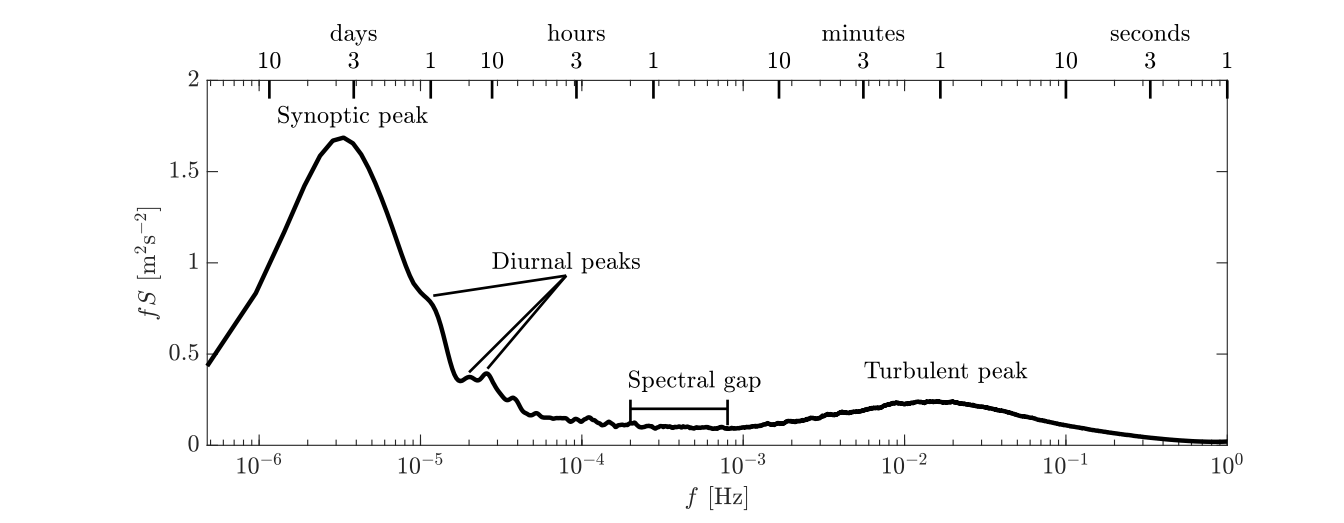
\includegraphics[width=\textwidth]{Figures/WindSpectra.png}
    \caption{Wind spectrum illustrating the distribution of energy across different frequencies at Bremerhaven measured by a cup anemometer
    at the height of 44 m \cite{Rettenmeier2013}.}
    \label{fig:windspectrum}
\end{figure}
As shown in Figure~\ref{fig:windspectrum}, the horizontal wind speed spectrum illustrates the distribution of energy across different frequencies. The synoptic peak is largely influenced by large-scale weather systems, while diurnal peaks arise from daily temperature variations between land and sea due to the day-night cycle. Between approximately 10 minutes and 1 hour, wind fluctuations tend to be minimal under normal conditions; this region is commonly referred to as the spectral gap. At higher frequencies—those associated with minute-scale variations—a distinct peak appears, which is linked to atmospheric turbulence.

In the context of modern wind turbines, high-frequency wind fluctuations are particularly significant because they often align with the natural frequencies of turbine structures, thereby contributing to fatigue loads. Conversely, low-frequency components of the spectrum are more relevant for understanding variations in power output and maintaining grid stability \cite{kosovic2025}. Due to the spectral gap, wind turbine design typically focuses on characterizing turbulent and mean wind components over time intervals of 10 to 30 minutes. Using longer intervals risks incorporating diurnal variations, which have little influence on turbine loading.

\subsection{Kaimal Spectrum}
The Kaimal spectrum is a widely used model to represent the energy distribution of turbulence in the atmospheric boundary layer. It provides a mathematical representation of the wind spectrum, particularly for horizontal wind speed fluctuations. The Kaimal spectrum is defined as:

\begin{equation}
S_u(f) = \frac{\sigma_u^2 L_u}{U} \frac{4fL_u/U}{\left(1 + 6fL_u/U\right)^{5/3}}
\end{equation}

where:
\begin{itemize}
    \item $S_u(f)$ is the power spectral density of the longitudinal wind speed fluctuations at frequency $f$,$\sigma_u$ is the standard deviation of the longitudinal wind speed fluctuations, $L_u$ is the integral length scale of turbulence in the longitudinal direction, $U$ is the mean wind speed, $f$ is the frequency.
\end{itemize}

The Kaimal spectrum captures the energy distribution across different frequencies, with the following characteristics:
\begin{itemize}
    \item At low frequencies, the spectrum exhibits a $f^{-1}$ behavior, indicating that large-scale eddies dominate the energy.
    \item At high frequencies, the spectrum follows a $f^{-5/3}$ decay, consistent with Kolmogorov's theory of turbulence for the inertial subrange.
\end{itemize}

This spectrum is particularly useful for wind turbine design, as it provides insights into the turbulent energy content at different scales, which directly impacts turbine loading and performance. Figure~\ref{fig:windspectrum} illustrates how the Kaimal spectrum aligns with the observed wind spectrum, highlighting its relevance in characterizing atmospheric turbulence.

The consistency between wind modeling approaches and actual measurement data supports the common practice of separating wind into mean components and turbulence spectra. Consequently, wind turbine simulations are typically conducted as follows: 

First, a series of turbulent wind fields—each 10 minutes long—are generated based on turbulence and vertical wind shear models for various mean wind speeds. According to \cite{iec61400}ng at least six simulations per mean wind speed, spaced at 2~m/s intervals from cut-in to cut-out speeds, is recommended to ensure statistically reliable results. Second, the wind speed distribution is modeled using a probability density function, which is then used to extrapolate and weight performance metrics such as power output, pitch activity, and structural loads over the turbine's operational lifetime.

The wind fields used in aero-elastic simulations are time series of three-dimensional wind velocity vectors defined at discrete points on a vertical, stationary, two-dimensional grid. In this study, wind fields are generated using \texttt{TurbSim}~\cite{ref57}, which applies a rectangular grid layout. These wind fields are then used in \texttt{FAST} for aero-elastic simulations, where they are interpolated along the rotating blades to compute aerodynamic forces and moments using the Blade Element Momentum (BEM) method, as described in Section \ref{sec:bem_theory}. 

Although the rotor plane can shift longitudinally due to nacelle motion or blade deflection, the wind field imported into \texttt{FAST} remains fixed and does not account for such movements.


The Kaimal spectrum, widely used in wind turbine load analysis, has notable limitations: it captures only second-order turbulence statistics, assumes Gaussian-distributed wind fluctuations (underestimating extreme events), and fails to represent intermittent, gusty features or heavy-tailed distributions observed in real atmospheric inflows. These shortcomings can lead to inaccuracies in predicting alternating loads on turbine components and discrepancies in torque statistics compared to real atmospheric data, potentially causing design and operational errors \cite{Mucke2011}.

A numerical flow model like Large Eddy Simulation(LES) is important compared to the Kaimal spectrum because it provides a more realistic and detailed representation of atmospheric turbulence. While the Kaimal model is limited to basic statistical properties and assumes Gaussian, stationary turbulence, numerical models solve the actual fluid dynamics equations, capturing complex and non-Gaussian features like gusts, ramps, and coherent structures. This allows for better prediction of loads and fatigue on wind turbines, especially in turbulent and complex terrains. Unlike the Kaimal model, numerical simulations offer spatial and temporal coherence, making them more suitable for modern applications like wake modeling, advanced turbine control, and site-specific assessments. \cite{Doubrawa2019}


\section{The Governing Equations of flow of motion}
\subsection{Navier-Stokes equations}
The motion of viscous fluids (e.g. the air flow over wind turbine blades) can be described by
means of the Navier-Stokes equations \cite{NSeqn}, which are based on the conservation of mass, momentum
and energy. The energy equation is disregarded in this thesis, since it is only required for
compressible flows (compressible effects are negligible in wind turbines since Ma < 0.3). The
Navier-Stokes equations assuming constant density can be written in differential, scalar form
as:
\begin{definition}[Navier Stokes Equations] \label{def:NSeqn}
    \textbf{Conservation of Mass:}
    The conservation of mass, also known as the continuity equation, ensures that mass is neither
    created nor destroyed. For an incompressible fluid, this is expressed as:
    \begin{equation}
    \nabla \cdot \mathbf{u} = 0
    \end{equation}
    where $\mathbf{u}$ is the velocity vector of the fluid.
    
    \textbf{Conservation of Momentum:}
    The conservation of momentum describes how the velocity of the fluid changes due to forces acting on it. For an incompressible fluid, the Navier-Stokes momentum equation is:
    \begin{equation}
    \rho \left( \frac{\partial \mathbf{u}}{\partial t} + \mathbf{u} \cdot \nabla \mathbf{u} \right) = -\nabla p + \mu \nabla^2 \mathbf{u} + \mathbf{f}
    \end{equation}
    where:
    \begin{itemize}
        \item $\rho$ is the fluid density (assumed constant), $\mathbf{u}$ is the velocity vector, $p$ is the pressure, $\mu$ is the dynamic viscosity, $\mathbf{f}$ represents external body forces (e.g., gravity, coriolis forces).
    \end{itemize}
    For detailed information on the Navier-Stokes equations, refer to \cite{NSeqn}
\end{definition}



\subsection{Turbulence Modeling}

Turbulence modeling is essential for understanding and simulating fluid flows at high Reynolds numbers. At low Reynolds numbers, the flow is laminar, with smooth and orderly motion. However, at high Reynolds numbers, the flow becomes turbulent, characterized by chaotic velocity and pressure fluctuations. These fluctuations result in increased mixing and diffusion of mass, momentum, and energy.

Turbulent flows exhibit an energy cascade, where large eddies extract energy from the mean flow and transfer it to smaller eddies through vortex stretching. This process continues until the smallest eddies dissipate energy into heat due to viscous effects.

The transition to turbulence is often triggered by flow instabilities in sheared flows. These instabilities amplify, leading to the formation of rotational structures and fully turbulent flows. To simulate turbulent flows, various strategies are employed, including Direct Numerical Simulation (DNS), Reynolds-Averaged Navier-Stokes (RANS), and Large Eddy Simulation (LES), each with its own trade-offs in accuracy and computational cost.

\subsection{Direct Numerical Simulation (DNS) and its limitations:}
Direct Numerical Simulation (DNS) involves solving the Navier-Stokes equations without any turbulence modeling, 
resolving all scales of motion down to the smallest eddies. While DNS provides highly accurate results, 
it is computationally prohibitive for most practical engineering applications, including wind turbines.

The computational cost of DNS scales with the Reynolds number ($Re$) as $Re^{3}$ to $Re^{3.5}$, 
due to the need to resolve the smallest turbulent scales. For wind turbines, the Reynolds number is typically in the range of $10^6$ to $10^7$, 
making DNS infeasible. Furthermore, the use of DNS also requires very accurate, low-dissipative numerical schemes
\cite{mocket2009}. This makes this type of simulation unsuitable for most technical applications,
especially for high Reynolds number flows. According to \cite{spalart2000}, the computational
power required for simulating an aircraft by means of CFD will not be readily available before
the year 2080. However, DNS is already used for performing basic turbulence research at low
Reynolds numbers 
Additionally, the large physical domain of wind turbine simulations, which includes the rotor blades and the surrounding atmospheric boundary layer, 
\subsection{Reynolds-Averaged Navier-Stokes (RANS) Equations}
To address the computational challenges of Direct Numerical Simulation (DNS), the Reynolds-Averaged Navier-Stokes (RANS) equations are commonly used. The RANS approach involves decomposing the instantaneous velocity and pressure fields into mean and fluctuating components:

\begin{equation}
\mathbf{u} = \overline{\mathbf{u}} + \mathbf{u}'
\end{equation}
\begin{equation}
p = \overline{p} + p'
\end{equation}

where:
\begin{itemize}
    \item $\overline{\mathbf{u}}$ and $\overline{p}$ are the mean velocity and pressure fields, $\mathbf{u}'$ and $p'$ are the fluctuating components of velocity and pressure.
\end{itemize}

Substituting these decompositions into the Navier-Stokes equations and applying a time-averaging operation results in the RANS equations:
\textbf{Reynolds-Averaged Navier-Stokes (RANS) Equations:}

\textbf{Conservation of Mass:}
\begin{equation}
\nabla \cdot \overline{\mathbf{u}} = 0
\end{equation}

\textbf{Conservation of Momentum:}
\begin{equation}
\rho \left( \frac{\partial \overline{\mathbf{u}}}{\partial t} + \overline{\mathbf{u}} \cdot \nabla \overline{\mathbf{u}} \right) = -\nabla \overline{p} + \mu \nabla^2 \overline{\mathbf{u}} - \nabla \cdot \overline{\mathbf{u}' \mathbf{u}'}
\end{equation}

Here, the Reynolds stress tensor $\overline{\mathbf{u}' \mathbf{u}'}$ is defined as:
\begin{equation}
\overline{\mathbf{u}' \mathbf{u}'} = 
\begin{bmatrix}
\overline{u'^2} & \overline{u'v'} & \overline{u'w'} \\
\overline{v'u'} & \overline{v'^2} & \overline{v'w'} \\
\overline{w'u'} & \overline{w'v'} & \overline{w'^2}
\end{bmatrix}
\end{equation}

The term $\overline{\mathbf{u}' \mathbf{u}'}$ represents the Reynolds stresses, 
which account for the effects of turbulence on the mean flow. 
These stresses introduce additional unknowns, making the system of equations unclosed. 
To close the RANS equations, turbulence models such as the $k$-$\epsilon$ or $k$-$\omega$ models are used to approximate the Reynolds stresses.

RANS has the advantage of being computationally efficient and widely validated, making it suitable for many engineering applications where time-averaged solutions are sufficient.
However, its reliance on turbulence models introduces approximations, which can reduce accuracy for flows with strong unsteadiness, separation, or complex turbulence structures.

\subsection{Large Eddy Simulation (LES)}
Large Eddy Simulation (LES) is a numerical technique used to simulate turbulent flows by resolving the large-scale turbulent structures 
while modeling the effects of smaller, sub-grid scale (SGS) motions. LES bridges the gap between Direct Numerical Simulation (DNS) 
and Reynolds-Averaged Navier-Stokes (RANS) by providing a balance between computational cost and accuracy.

In atmospheric flows Large Scale eddies contain more energy and transport moreeffectively the 
momentum and scalars than the small scale eddies\cite{spalart2000}. Thats why putting
more computational effort on the large scale eddies is more efficient than putting it on the small scale eddies and it 
does not severely comprimise simulation accuracy. Furthermore, modelling the small scale turbulence is comparatively simple because of
its isotropic, homogeneous and universal characteristics (in opposition to the anisotropic and
anisotropic problem-specific characteristics of large scale turbulence).
The LES approach involves applying a spatial filtering operation to the Navier-Stokes equations,
which separates the flow field into resolved (large-scale) and unresolved (small-scale) components.
The filtering operation is defined as: 
\begin{equation}
\overline{\phi}(\mathbf{x}, t) = \int_V \phi(\mathbf{x}', t) G(\mathbf{x} - \mathbf{x}') d\mathbf{x}'
\end{equation}
where:
\begin{itemize}
    \item $\phi$ is a flow variable (e.g., velocity, pressure), $G$ is the filter function, which determines the scale of the resolved motions, $V$ is the volume of the computational domain.
\end{itemize}

Different types of filter exist, but all of them have in common the
usage of a length scale $\Delta$ which is the filter width. The filter width
is the characteristic length scale of the large eddies that are resolved in the simulation.
The filter function $G$ is typically chosen to be a Gaussian or box filter,
which allows for the separation of large and small scales. The filter width $\Delta$ is a critical parameter that determines the scale of the resolved motions in the simulation.

Applying the filtering operation to the Navier-Stokes equations results in the filtered equations of motion:

\textbf{Filtered Conservation of Mass:}
\begin{equation}
\nabla \cdot \overline{\mathbf{u}} = 0
\end{equation}

\textbf{Filtered Conservation of Momentum:}
\begin{equation}
\rho \left( \frac{\partial \overline{\mathbf{u}}}{\partial t} + \overline{\mathbf{u}} \cdot \nabla \overline{\mathbf{u}} \right) = -\nabla \overline{p} + \mu \nabla^2 \overline{\mathbf{u}} - \nabla \cdot \tau_{SGS}
\end{equation}
where $\tau_{SGS}$ is the sub-grid scale stress tensor, defined as:
\begin{subequations}
    \begin{equation}
    \tau_{SGS} = \overline{\mathbf{u} \mathbf{u}} - \overline{\mathbf{u}} \, \overline{\mathbf{u}}
    \end{equation}
\end{subequations}
    

The sub-grid scale stress tensor $\tau_{SGS}$ represents the effects of the unresolved small-scale motions on the resolved large-scale motions. To close the LES equations, $\tau_{SGS}$ must be modeled using a sub-grid scale model.

\textbf{Sub-Grid Scale Models:}
There are two widely used methods to approximate $\tau_{SGS}$. Those models are:

1. \textbf{Smagorinsky Model:}
   The Smagorinsky model assumes that the SGS stresses are proportional to the strain rate of the resolved flow:
   \begin{equation}
   \tau_{SGS} = -2 \nu_t \mathbf{S}
   \end{equation}
   where:
   \begin{itemize}
       \item $\nu_t = (C_s \Delta)^2 |\mathbf{S}|$ is the eddy viscosity, $C_s$ is the Smagorinsky constant (typically $C_s \approx 0.1$), $\Delta$ is the filter width, $\mathbf{S}$ is the strain rate tensor, defined as $\mathbf{S} = \frac{1}{2} \left( \nabla \overline{\mathbf{u}} + \nabla \overline{\mathbf{u}}^T \right)$.
   \end{itemize}

2. \textbf{Dynamic Smagorinsky Model:}
   The dynamic Smagorinsky model improves upon the Smagorinsky model by dynamically computing the Smagorinsky constant $C_s$ based on the local flow conditions. 
   This is achieved by applying a second filtering operation (test filter) and using the Germano identity to determine $C_s$.
    The dynamic Smagorinsky model is more adaptive to varying flow conditions and provides better results in complex flows.

LES provides a detailed representation of turbulent flows, capturing the energy-containing large eddies while modeling the dissipative small scales. It is widely used in engineering and scientific applications where DNS is computationally infeasible, and RANS lacks sufficient accuracy. In the present work the
large-eddy simulation (LES) tool PALM \cite{maronga2015}, developed at the Institute for Meteorology and
Climatology (IMUK) of Leibniz University Hannover is used. 

The PALM model is built upon the non-hydrostatic, filtered, incompressible Navier–Stokes equations, formulated using the Boussinesq approximation. An anelastic approximation is also available as an option for simulating deep convection. By default, PALM solves for at least six prognostic variables: the three velocity components ($u$, $v$, $w$) on a Cartesian grid, the potential temperature ($\theta$), the water vapor mixing ratio ($q_v$), and optionally a passive scalar ($s$). Additionally, a prognostic equation is solved either for the subgrid-scale turbulent kinetic energy (SGS-TKE, $e$) in large-eddy simulation (LES) mode—used by default—or for the total turbulent kinetic energy in Reynolds-averaged Navier–Stokes (RANS) model.

In LES mode, the filtering operation introduces four subgrid-scale (SGS) covariance terms, which are parameterized using a 1.5-order turbulence closure following Deardorff (1980). PALM employs a modified version of the closure schemes proposed by Moeng and Wyngaard (1988) and Saiki et al. (2000). This closure assumes that the energy transport by SGS eddies is proportional to the local gradients of the resolved flow variables.

A comprehensive description of PALM and its functionalities can be found in the official PALM documentation and related publications\cite{maronga2015} \cite{raasch2001}.

\chapter{Numberics governing Aeroelastic Simulation of a Wind Turbine}
\section{Aeroelastic Simulation of a Wind Turbine}

\subsection{Blade Element Momentum (BEM) Theory} 
\label{sec:bem_theory}

Wind turbines are commonly modeled using aeroelastic simulation tools, which provide reliable system-level accuracy and are widely used in certification procedures. The Blade Element Momentum (BEM) theory is a widely used method for analyzing the aerodynamic performance of wind turbine blades. It combines two fundamental principles: the blade element theory and the momentum theory. These equations can be solved iteratively under the assumption that aerodynamic interactions between blade elements are negligible \cite{ingram2011blade}. The first approach, known as Momentum Theory, is based on applying force and momentum balance to an annular streamtube. The second, Blade Element Theory, calculates lift and drag forces at discrete sections along the blade.
\subsubsection{Momentum Theory}
Consider a streamtube surrounding a wind turbine rotor,
\begin{figure}[ht]
    \centering
    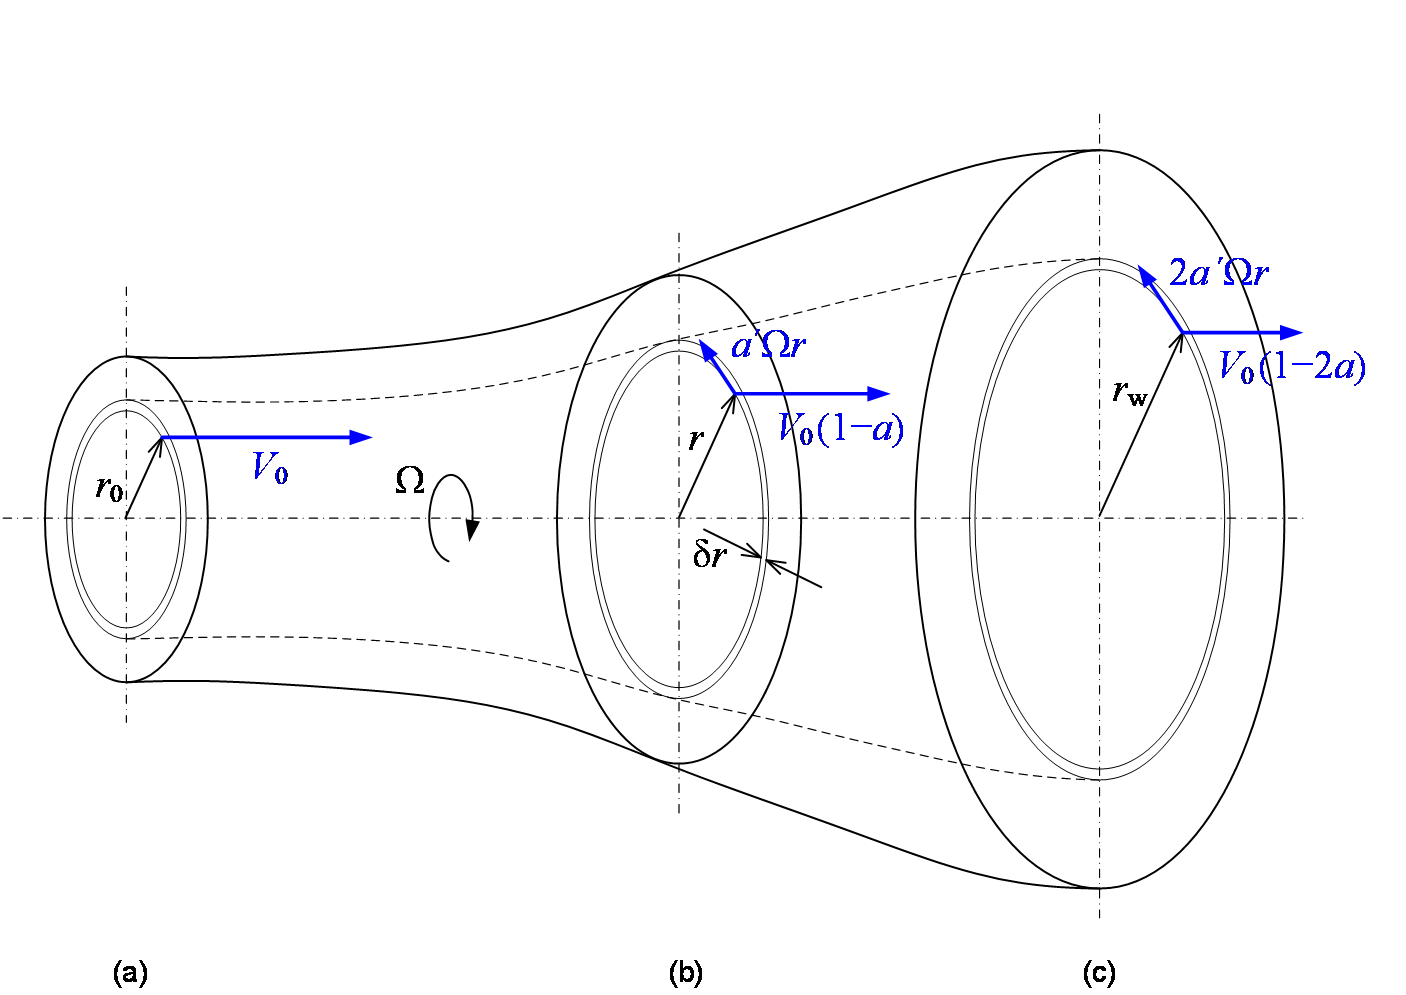
\includegraphics[width=\textwidth]{Figures/aerodynamics_streamtube.png}
    \caption{Streamtube around a wind turbine rotor.}
    \label{fig:streamtube}
\end{figure}


The axial force $dF_x$ and torque $dT$ on an annular element of a wind turbine rotor can be expressed as:

Axial Force:
\begin{equation}
dF_x = 4\pi \rho V_1^2 a(1 - a) r \, dr
\end{equation}

Tangential Force:
\begin{equation}
dT = 4\pi \rho a' (1 - a) \Omega V_1 r^3 \, dr
\end{equation}

Here, $a$ is the axial induction factor, $a'$ is the angular induction factor, $\rho$ is the air density, $V_1$ is the free-stream wind speed, $\Omega$ is the angular velocity of the rotor, $r$ is the radial position, and $dr$ is the thickness of the annular element. For detailed information on the BEM theory and its derivations, refer to \cite{ingram2011blade}.
\subsubsection{Blade Element Theory}
The blade element theory calculates the aerodynamic forces acting on a small element of the rotor blade. The lift and drag forces can be expressed as:
\begin{equation}
dF_L = \frac{1}{2} \rho V^2 C_L dA
\end{equation}
\begin{equation}
dF_D = \frac{1}{2} \rho V^2 C_D dA
\end{equation}

where:
\begin{itemize}
    \item $dF_L$ is the lift force, $dF_D$ is the drag force, $\rho$ is the air density, $V$ is the relative wind speed at the blade element, $C_L$ and $C_D$ are the lift and drag coefficients, respectively, and $dA$ is the area of the blade element.
\end{itemize}
The lift and drag coefficients are functions of the angle of attack ($\alpha$) and can be obtained from experimental data or empirical models. The angle of attack is defined as:
\begin{equation}
\alpha = \beta - \phi
\end{equation}
where:
\begin{itemize}
    \item $\beta$ is the pitch angle of the blade element, and $\phi$ is the angle between the relative wind direction and the chord line of the blade element.
\end{itemize}
The aerodynamic forces on a wind turbine blade segment depend on the lift and drag coefficients, $c_L(\alpha)$ and $c_D(\alpha)$, which vary with the angle of attack $\alpha$. The angle $\beta$ represents the inclination of the blade segment relative to the rotor plane, as illustrated in Figure~\ref{fig:blade_geometry}.

The differential aerodynamic thrust and torque on an annular ring can be expressed as:
\begin{align}
    dF_a &= n_B \left( dL_a \cos(\alpha + \beta) + dD_a \sin(\alpha + \beta) \right), \label{eq:thrust_force} \\
    dM_a &= n_B \left( dL_a \sin(\alpha + \beta) - dD_a \cos(\alpha + \beta) \right) r, \label{eq:torque}
\end{align}
where $n_B$ is the number of blades, $dL_a$ and $dD_a$ are the differential lift and drag forces, and $r$ is the radial position.
\begin{figure}[ht]
    \centering
    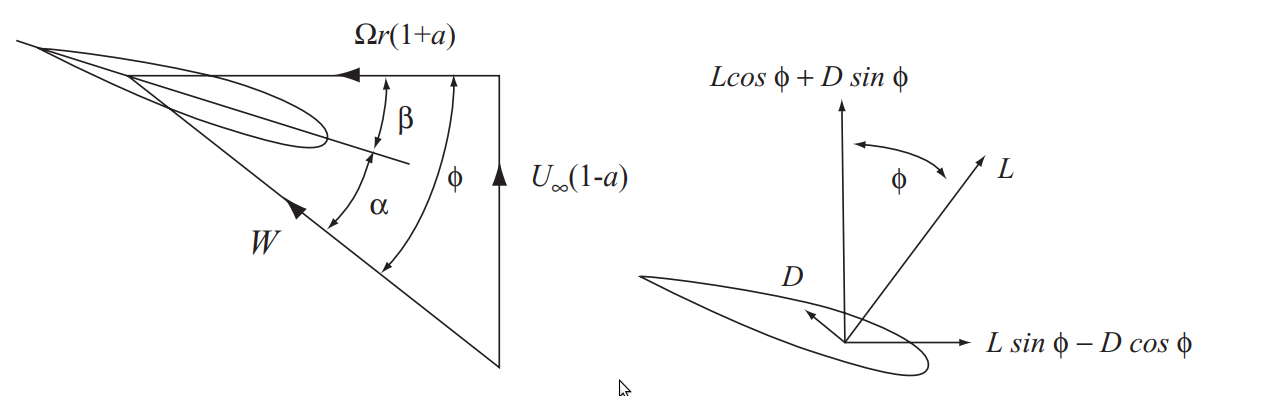
\includegraphics[width=\textwidth]{Figures/blade_element.png}
    \caption{Blade element velocities (left) and forces (right) \cite{burton2011}.}
    \label{fig:blade_geometry}
\end{figure}

From geometric considerations shown in Figure~\ref{fig:blade_geometry}, the inflow angle is given by:
\begin{equation}
    \tan(\alpha + \beta) = \frac{u_1(1 - a_{\text{ax}})}{\Omega r (1 + a_{\text{an}})},
\end{equation}
and the relative inflow speed is:
\begin{equation}
    v_{\text{inflow}}^2 = \left( \Omega r (1 + a_{\text{an}}) \right)^2 + \left( u_1 (1 - a_{\text{ax}}) \right)^2. \label{eq:inflow_speed}
\end{equation}

Equations~\eqref{eq:thrust_force} and~\eqref{eq:torque} are equated with the corresponding expressions from momentum theory to form a system of two nonlinear equations. The unknowns $a_{\text{ax}}$ (axial induction factor) and $a_{\text{an}}$ (angular induction factor) are then solved iteratively for each blade section, given known values of $u_1$, $\Omega$, $\rho$, $\beta$, $r$, $dr$, $c$, and the aerodynamic coefficients $c_L(\alpha)$ and $c_D(\alpha)$.
For detailed information on the Blade Element theory and its derivations, refer to \cite{ingram2011blade}.

The total aerodynamic thrust and torque are obtained by integrating $dF_a$ and $dM_a$ across all blade elements. The aerodynamic module of FAST implements these calculations along with empirical corrections such as tip and hub loss factors~\cite{fastV3}, enhancing the accuracy of the Blade Element Momentum (BEM) method.
         
\subsection{Structural Dynamics of Wind Turbines}

Wind turbine structural dynamics can be modeled using two main approaches: finite element (FE) models and modal analysis~\cite{bossanyi2010}. In practice, modal models with fewer Degrees of Freedom (DOFs) are often preferred due to their lower computational cost.

In this work, the FAST code is used to model the turbine structure. The structural equations are derived in a preprocessing step using \texttt{BModes}~\cite{bir2009}. The tower and blades are modeled as Euler-Bernoulli beams, which are discretized into multiple segments using finite element methods. This results in a system of nonlinear, coupled Ordinary Differential Equations (ODEs), capturing variations in mass, stiffness, and inertia along the structure.

These nonlinear equations are linearized, and an eigenvalue analysis is performed to extract the natural vibration modes. The resulting mode shapes $\mu_i(r)$, distributed mass, and stiffness properties are stored in input files for FAST. Each mode shape $\mu_i(r)$ is a polynomial in the radial position $r$ and is normalized such that $\mu_i(r_{\text{end}}) = 1$.

Assuming small deflections, a linear modal representation is used for blades and tower. For each mode $i$, the modal mass $m_i$, stiffness $k_i$, damping $c_i$, and external force $F_i$ are computed using:

\begin{align}
    m_i &= \sum_{j=1}^{n_S} m_j \mu_i^2(r_j), \label{eq:modal_mass} \\
    k_i &= \sum_{j=1}^{n_S} k_j \mu_i^2(r_j), \label{eq:modal_stiffness} \\
    c_i &= \frac{d_{s,i} k_i}{\pi f_{0,i}}, \quad f_{0,i} = \frac{1}{2\pi} \sqrt{\frac{k_i}{m_i}}, \label{eq:modal_damping} \\
    F_i &= \sum_{j=1}^{n_S} F_j \mu_i(r_j), \label{eq:modal_force}
\end{align}

where $d_{s,i}$ is the structural damping ratio, and $f_{0,i}$ is the natural frequency of mode $i$.

The equation of motion for a single mode is:

\begin{equation}
    m_i \ddot{q}_i + c_i \dot{q}_i + k_i q_i = F_i. \label{eq:single_mode_eom}
\end{equation}

In FAST, each blade is modeled using the first edgewise mode and the first two flapwise modes. The tower is modeled with the first two modes in both fore-aft and side-to-side directions. Including rotor rotation, drive train torsion, and nacelle yaw, this results in a total of 16 DOFs for a three-bladed wind turbine.

The total deflection of a flexible component is reconstructed by superimposing all mode shapes weighted by the current modal amplitudes. The coupled equations of motion are derived using Kane’s method~\cite{kane1985}, which accounts for nonlinear interactions between structural and rotational DOFs. For example, tower motion depends on the instantaneous azimuthal positions of the blades. Rotor speed also affects mode frequencies due to centrifugal stiffening.

The complete system of equations is written in the general form:

\begin{equation}
    \mathbf{M}(\mathbf{q}, \mathbf{u}) \ddot{\mathbf{q}} + \mathbf{f}(\mathbf{q}, \dot{\mathbf{q}}, \mathbf{u}, \mathbf{d}) = 0, \label{eq:general_eom}
\end{equation}

where $\mathbf{q}$ is the vector of modal coordinates, $\mathbf{u}$ represents control inputs, and $\mathbf{d}$ includes external disturbances such as wind loads.

\section{Numerical Flow model of a Wind Turbine}
\subsection{The Actuator Line Model} 

The Actuator Line Model (ALM) is a numerical approach used to simulate the aerodynamic forces exerted by wind turbine blades on the surrounding flow field. In this model, the blades are represented as lines of discrete force elements rather than as solid surfaces. These force elements are distributed along the span of the blade and are computed based on the local flow conditions and the blade's aerodynamic properties. The ALM captures the unsteady aerodynamic interactions between the blades and the turbulent flow, making it suitable for high-fidelity simulations of wind turbine wakes and rotor dynamics. The forces are smoothed using a Gaussian kernel to avoid numerical instabilities and to account for the finite resolution of the computational grid. This smoothing ensures that the aerodynamic forces are distributed over a small region around the actuator line, rather than being concentrated at discrete points.

The ALM is computationally efficient compared to fully resolved blade simulations, as it eliminates the need to resolve the blade geometry explicitly. However, it requires accurate input data, such as airfoil characteristics and blade geometry, to ensure reliable results. The model is widely used in Large Eddy Simulations (LES) of wind farms, where it provides detailed insights into wake interactions and turbulence effects.
\subsection{The Actuator Disk Model} 
The Actuator Disk Model (ADM) is a simplified approach for simulating the aerodynamic effects of a wind turbine rotor on the flow field. In this model, the rotor is represented as a permeable disk that exerts a uniform or spatially varying force distribution on the incoming flow. The ADM is based on the principles of momentum theory and assumes that the rotor induces a pressure drop and velocity deficit in the flow, which are proportional to the thrust and power coefficients of the turbine. The ADM is computationally less demanding than the Actuator Line Model, as it does not require detailed blade geometry or airfoil data. It is particularly useful for large-scale simulations of wind farms, where the focus is on the overall flow dynamics rather than the detailed blade aerodynamics. However, the ADM lacks the ability to capture unsteady blade-wake interactions and the effects of blade-specific aerodynamic features. Despite these limitations, the ADM remains a valuable tool for studying wind farm performance, wake interactions, and optimization strategies in scenarios where computational resources are limited.
\subsection{The Actuator Sector Model} 
\begin{tikzpicture}[scale=1.2]

    % Common settings
    \def\towerHeight{6}
    \def\towerBaseX{0}
    \def\towerTopX{0.2}
    
    % Title
    \node at (2.5,7.5) {\Large Modal Shapes of a Wind Turbine};
    
    %%%% First Mode Shape (Bending)
    \node[above] at (0,6.5) {\textbf{1st Mode: Bending (Fore-Aft)}};
    
    % Base line
    \draw[thick] (0,0) -- (0,6);
    
    % Mode shape
    \draw[very thick, blue] plot[smooth] coordinates {
        (0,0)
        (0.05,1)
        (0.1,2)
        (0.15,3)
        (0.2,4)
        (0.25,5)
        (0.3,6)
    };
    
    % Nacelle
    \draw[fill=gray] (0.3,6) circle (0.15);
    \draw[->, thick] (0.3,6) -- +(0.8,0) node[right] {Blades};
    
    %%%% Second Mode Shape (S-Shaped)
    \node[above] at (5,6.5) {\textbf{2nd Mode: S-Bending}};
    
    % Base line
    \draw[thick] (4,0) -- (4,6);
    
    % Mode shape
    \draw[very thick, red] plot[smooth] coordinates {
        (4,0)
        (3.95,1)
        (4.05,2)
        (3.95,3)
        (4.05,4)
        (3.95,5)
        (4.1,6)
    };
    
    % Nacelle
    \draw[fill=gray] (4.1,6) circle (0.15);
    \draw[->, thick] (4.1,6) -- +(0.8,0) node[right] {Blades};
    
    \end{tikzpicture}


\chapter{Summary} \label{cha:SUM}


\backmatter
%% NOTE: uncomment following line if you use parts in your document
% \addtocontents{toc}{\vspace{2ex}}  % Add extra space after the last part in TOC

\chapternotnumbered{Summary and Outlook}

Summary and Outlook.


\appendix
\addcontentsline{toc}{chapter}{Appendix}
\chapter{Heading Appendix A} \label{app:A}


\chapter{Heading Appendix B} \label{app:B}

\chapter{Heading Appendix C}


\references

\end{document}
